% =========================================================================
% Chapter 8 — Causal Identification via CBAM: A Multi-Source Triangulation
% Sake Saakstra, MSc EOR Financial Track, Vrije Universiteit Amsterdam
% Supervisor: prof. dr. S.J. Koopman | Second reader (proposed): dr. N. Ketel
% Version: v1, 19 May 2026
% =========================================================================
\documentclass[11pt,a4paper]{article}

\usepackage[a4paper,margin=2.5cm]{geometry}
\usepackage{amsmath,amssymb,amsthm,bm}
\usepackage{graphicx}
\usepackage{booktabs}
\usepackage{natbib}
\usepackage{hyperref}
\usepackage[table]{xcolor}
\usepackage{caption}
\hypersetup{colorlinks=true,linkcolor=blue!50!black,citecolor=blue!50!black,urlcolor=blue!50!black}

\newcommand{\bint}{\beta_{\mathrm{int}}}
\newcommand{\bcbam}{\beta_{\mathrm{CBAM}}}
\newcommand{\bep}{\beta_{\mathrm{EP}}}
\newcommand{\E}{\mathbb{E}}
\newcommand{\indicator}{\mathbb{1}}

\title{\textbf{Chapter 8 — Causal Identification via the Carbon Border Adjustment Mechanism}\\[0.4em]
\large A Multi-Source Triangulation of the Carbon-Conditional Hydrogen Cancellation Mechanism}
\author{Sake Saakstra \\ \small Vrije Universiteit Amsterdam, MSc Econometrics \& Operations Research (Financial Track) \\ \small Supervisor: prof.\ dr.\ S.J.\ Koopman \\ \small Second reader (proposed): dr.\ N.\ Ketel}
\date{Version 1, 19 May 2026}

\begin{document}
\maketitle

\begin{abstract}
\noindent Chapters 5--7 established a robust associational relationship between EUA prices and the differential Blue-versus-PEM hydrogen project cancellation hazard, with the time-varying interaction parameter $\bint$ ranging from $-1.17$ to $-1.88$ across specifications. This chapter exploits the European Union's Carbon Border Adjustment Mechanism (CBAM), which entered its definitive financial-obligation phase on 1 January 2026, as a sudden, plausibly exogenous shock to test whether this relationship reflects a causal mechanism. We deploy three independent data sources (the curated v7 sample with 714 projects and 43 cancellation events; the S\&P Global Hydrogen Master Data Table with 3{,}343 projects, daily refresh; and the IEA Hydrogen Production Projects Database with 2{,}625 projects and multi-checkbox end-use classification) and four identification strategies (equity event study with placebo-corrected difference-in-differences; project-level vintage cohort difference-in-differences; EU-restricted placebo-rich difference-in-differences with five placebo treatment dates; and a triple-difference combining geographic and sectoral exposure). All four strategies return informative nulls. We document a robust associational pattern across both S\&P and IEA: CBAM-end-use exposed projects in the EU-27 face $+17$ to $+20$ percentage points higher cancellation (or equivalent reduction in advanced-status probability) than non-exposed comparators, while the opposite holds outside the EU. However, placebo treatment dates within the EU sample produce coefficient estimates of equal or greater magnitude than the real CBAM dates (real/placebo ratio $0.72$), and a triple-difference EU $\times$ CBAM $\times$ post-2022 specification yields $\beta = +1.15$ with 95\% credible interval $[-1.48, +3.78]$. We interpret these results in the framework of \citet{ketel2023unimportance}: a methodologically informative null whose contribution is to bound the magnitude of any causal CBAM channel and to demonstrate that the observed differential cannot be attributed to a single policy treatment. We discuss three substantive interpretations (anticipation effects, structural EU-specific industrial-conversion difficulties, and insufficient power) and conclude with implications for the thesis's overall claim regarding the carbon-conditional differential cancellation mechanism.
\end{abstract}

\tableofcontents
\newpage

% =========================================================================
\section{Introduction and Motivation}
\label{sec:ch8-intro}

\subsection{The empirical puzzle from Chapters 5--7} Within the broader implementation-risk framework of this thesis, the present chapter probes whether observed cancellation patterns can be causally attributed to a specific regulatory shock; we conclude with what we term an \textit{informative null}.

The body of empirical evidence assembled in Chapters 5 through 7 establishes a robust pattern: hydrogen projects employing blue (gas-with-CCS) technologies exhibit cancellation hazards that respond differentially to carbon prices, with the time-varying interaction parameter $\bint$ remaining negative across all specifications. Across pooled, sponsor-controlled, regional, and time-varying parameter (TVP) specifications, the point estimates cluster within the range $[-1.17, -1.88]$, with the gradual intensification documented in Chapter 6 (from $-0.73$ in 2014 to $-1.87$ in 2024) corroborated by a complementary equity event study showing $\gamma_{\mathrm{EUA}} = +0.041$ for diversified oil majors versus a null effect for PEM pure-plays. The Dixit--Pindyck-style real options framework developed in Chapter 3 rationalizes this pattern theoretically: when carbon prices rise, the option-to-defer becomes more valuable for projects whose marginal cost is carbon-elastic, and Blue projects are precisely the cases where this elasticity is high.

\subsection{The causal question}

The associational evidence is robust to multiple specifications, sponsor identification controls, geographic stratification, and time-varying parameter dynamics. What remains is the causal question: \emph{is the observed differential cancellation hazard the consequence of carbon-pricing exposure, or is it an artefact of unobserved factors that correlate with both Blue technology selection and project failure?} The Inflation Reduction Act DiD presented in Chapter 7 Section 7.6 yielded $\beta_{\mathrm{IRA}} = -0.15$ with credible interval $[-1.9, +1.5]$, an informative null that we attributed at the time to limited post-treatment events and to the IRA's protracted implementation timeline (final Treasury rules on the 45V credit only emerged in January 2025).

\subsection{Why CBAM provides the sharpest available test}

The EU's Carbon Border Adjustment Mechanism offers a substantially cleaner natural experiment than the IRA along three dimensions. First, the policy timeline contains discrete, well-documented treatment dates: regulation enters force on 18 April 2023, the transitional reporting-only phase begins on 1 October 2023, and the definitive financial-obligation phase commences on 1 January 2026 \citep{ec2023cbam}. Second, the policy mechanism is mechanically well-defined: importers of covered goods (cement, aluminium, fertilizers, iron and steel, hydrogen, and electricity) must surrender CBAM certificates priced at the prevailing EUA spot rate, thereby raising the effective carbon cost of hydrogen-derived products that enter the EU market. Third, in contrast to the IRA's politically uncertain implementation, the news evidence assembled in Section \ref{sec:ch8-institutional} demonstrates that the CBAM has produced observable real-economy responses already, including the BP Teesside Blue hydrogen withdrawal of December 2025 and the European Commission's March 2026 decision not to suspend CBAM for hydrogen-based fertilizers despite explicit industry lobbying.

\subsection{Scope of this chapter}

The contribution of this chapter is fourfold. First, we provide an explicit pre-registered identification design (Section \ref{sec:ch8-identification}) that follows the sudden-shock event-study framework of \citet{hanemaaijer2024minority}. Second, we deploy three independent data sources (Section \ref{sec:ch8-data}), each with different cancellation definitions, treatment timing availability, and end-use classification rigour, in order to triangulate the empirical pattern. Third, we run four distinct identification strategies (Sections \ref{sec:ch8-equity}--\ref{sec:ch8-triplediff}), each pre-registered with its own placebo and falsification suite. Fourth, we document the resulting set of informative nulls (Section \ref{sec:ch8-discussion}) in the methodological tradition of \citet{ketel2023unimportance}, and discuss three substantively different interpretations of the null pattern.

% =========================================================================
\section{Institutional Background and Treatment Timeline}
\label{sec:ch8-institutional}

\subsection{CBAM policy structure}

The Carbon Border Adjustment Mechanism is the European Union's response to the carbon-leakage concern: that domestic decarbonisation imposing carbon costs on EU producers may simply shift carbon-intensive production to jurisdictions with weaker climate policy. The regulation, formally Regulation (EU) 2023/956, was politically agreed in December 2022 and entered into force in April 2023. Three temporal milestones define the treatment timeline:

\begin{enumerate}
\item \textbf{Regulation entry-into-force (April 2023):} EU member states and importers receive formal legal certainty that CBAM will apply.
\item \textbf{Transitional phase (October 2023):} Importers of covered goods must report quarterly on the embedded emissions, but no financial obligation is imposed. The transitional phase is information-only.
\item \textbf{Definitive phase (January 2026):} Importers must purchase and surrender CBAM certificates equivalent to the embedded emissions of covered goods, at prices reflecting the EUA spot rate.
\end{enumerate}

\subsection{Coverage relevant to the hydrogen sector}

The CBAM's interaction with the hydrogen sector operates through three channels. First, hydrogen-based fertilizers (urea, ammonium nitrate) entered direct CBAM coverage from January 2026, exposing fertilizer producers selling into the EU market to certificate obligations proportional to their hydrogen-derived emissions intensity. Second, downstream sectors that consume hydrogen as an input -- iron and steel, aluminium, and (from 2027) chemicals -- carry their own phased CBAM obligations, indirectly raising the demand for low-carbon hydrogen inputs while simultaneously exposing CBAM-importing hydrogen-consuming projects to certificate costs. Third, Blue hydrogen production using imported natural gas (Norwegian, Algerian, US LNG, and Russian sources) may face indirect CBAM exposure through the carbon intensity of the upstream gas supply, even where hydrogen itself is not directly covered.

\subsection{Observed real-economy responses in the first four months}

The news evidence compiled for this chapter documents at least three categories of post-CBAM-launch responses. First, the European Commission's March 2026 decision not to suspend CBAM for hydrogen-based fertilizers signals political commitment to the policy and removes a key uncertainty that could have attenuated price pass-through \citep{ec2026hydrogen}. Second, multiple Blue hydrogen project withdrawals have occurred in the immediate run-up to and following the definitive phase: BP's Teesside Blue hydrogen Development Consent Order withdrawal of 1 December 2025; Exxon Mobil's pause of the Baytown Blue hydrogen-ammonia plant in November 2025 (formally citing offtake difficulties for export into the CBAM-exposed European fertilizer market); the cancellation of the Equinor-Linde H2M Eemshaven project in February 2026; and the ArcelorMittal Germany green hydrogen steel programme shelved with explicit CBAM-context references in March 2026. Third, the EU Hydrogen Bank's second auction round in September 2025 saw seven previously-awarded projects withdraw their applications (four in Spain, two in Germany, one in the Netherlands), suggesting that the convergence of REPowerEU subsidy uncertainty and CBAM-driven demand expectations was insufficient to maintain project economics.

% =========================================================================
\section{Identification Design and Pre-Registration}
\label{sec:ch8-identification}

\subsection{Treatment definitions}

Following the sudden-shock framework of \citet{hanemaaijer2024minority}, we pre-register three treatment definitions of increasing specificity, in order to bracket the channel through which CBAM may operate:

\paragraph{T1 (Narrow, end-use exposure).} A project is treated if its hydrogen output is destined for a downstream sector that is directly CBAM-covered. Operationally, T1 is satisfied if the S\&P field \texttt{Primary end use sector detail} or the IEA multi-checkbox indicates one of the following: fertilizer/ammonia, iron and steel, chemicals/methanol, oil refinery feedstock, or cement. T1 maps directly to the CBAM coverage list of Regulation (EU) 2023/956.

\paragraph{T2 (Broad, geographic-or-export OR end-use).} A project is treated under T2 if it satisfies T1, OR if it is located within the EU-27 customs union, OR if its export destination geography includes EU member states. T2 captures projects that compete with CBAM-exposed products in the EU market even where the primary end-use is not directly CBAM-covered.

\paragraph{T3 (Strict intersection).} A project is treated under T3 only if it satisfies both T1 (CBAM-covered end-use) and the geographic/export condition (located in EU-27 or exports to EU). T3 represents the cleanest identification, restricting attention to projects whose hydrogen output should be most directly affected by CBAM-induced demand or cost dynamics.

\subsection{Empirical specifications}

\paragraph{Specification 1 (Equity event study DiD).} For each candidate treatment date $t^*$, we estimate the cumulative abnormal returns (CAR) of treated and control equity portfolios over the event window $[-10, +20]$ trading days, following the standard CAPM-based event-study methodology. The difference-in-differences correction compares real treatment dates with placebo treatment dates of equal seasonality (one-year-prior placebos) to net out January-seasonal effects in cyclical sectors.

\paragraph{Specification 2 (Project-level vintage difference-in-differences).} On the project-level panel, we estimate the discrete-time logit hazard:
\begin{equation}
\Pr(\text{cancel}_{it}) = \Lambda\left(\alpha + \beta_1 \text{Treated}_i + \beta_2 \text{Post}_t + \bep (\text{Treated} \times \text{Post})_{it} + \gamma X_{it}\right),
\label{eq:ch8-did}
\end{equation}
where $\Lambda(\cdot)$ is the logistic CDF, $\text{Treated}_i$ takes T1, T2, or T3 depending on the specification, $\text{Post}_t$ indicates whether the project's announcement year is on or after the candidate treatment date, and $X_{it}$ contains controls for technology (Blue/PEM), log-capacity, and project-age covariates. The coefficient of interest is $\bep$, with statistical inference based on cluster-robust standard errors at the project level.

\paragraph{Specification 3 (EU-restricted placebo-rich DiD).} The specification above is re-estimated on the EU-27 sub-sample, with five placebo treatment dates (announcement-year cutoffs at 2015, 2017, 2019, 2020, 2021) used to bound any general announcement-vintage trend. The identifying assumption is that, conditional on the controls, the CBAM-exposure effect should appear at the true treatment dates (2022, 2023) but not at the placebo dates.

\paragraph{Specification 4 (Triple-difference, EU $\times$ CBAM $\times$ Post).} To formally test whether the EU-specific pattern documented in Chapter 7 Section 7.5 (the so-called EU paradox) reflects a CBAM-causal mechanism rather than a structural EU-specific factor, we estimate the saturated triple-difference:
\begin{align}
\Pr(\text{cancel}_{it}) = \Lambda(\alpha &+ \beta_1 \text{EU}_i + \beta_2 \text{CBAM-end}_i + \beta_3 \text{Post}_t \nonumber \\
&+ \beta_4 (\text{EU} \times \text{CBAM-end})_i + \beta_5 (\text{EU} \times \text{Post})_{it} + \beta_6 (\text{CBAM-end} \times \text{Post})_{it} \nonumber \\
&+ \boldsymbol{\beta_7} (\text{EU} \times \text{CBAM-end} \times \text{Post})_{it} + \gamma X_{it}).
\label{eq:ch8-triplediff}
\end{align}
The coefficient $\beta_7$ identifies the differential CBAM-effect on EU-located CBAM-end-use projects, conditional on the marginal main and pairwise interaction effects. Under the null hypothesis that the EU paradox reflects a structural pattern unrelated to CBAM, $\beta_7$ should be statistically indistinguishable from zero.

\subsection{Identifying assumptions and threats}

The identification of \eqref{eq:ch8-did}--\eqref{eq:ch8-triplediff} rests on three assumptions, each of which we test where possible.

\paragraph{A1 (Conditional parallel trends).} Conditional on the controls $X_{it}$, treated and control units would have followed parallel cancellation trajectories absent CBAM. This is tested via placebo treatment dates in Specification 3 and via the pattern of the pairwise interaction $\beta_6$ in Specification 4.

\paragraph{A2 (No confounding contemporaneous shocks).} The identification is threatened by other policy events affecting CBAM-exposed and non-exposed projects differentially in the same window. The most plausible confound is the IRA-driven re-shoring of hydrogen production toward North America, which would shift the CBAM-exposed (EU-located) sample relative to non-CBAM-exposed (North American) sample. We address this by including region-fixed effects and by examining the pattern within the EU-27 sub-sample (Specification 3).

\paragraph{A3 (Stable Unit Treatment Value, SUTVA).} The effect of CBAM on any given project does not depend on the treatment status of other projects. This is plausible at the project level (Blue and PEM projects do not directly cannibalise each other), but may be threatened at the sector-aggregate level if CBAM induces sector-wide rebalancing.

\subsection{Pre-registration commitments}

To pre-empt the most common reviewer concerns about ex-post specification mining, we commit ex ante to the following: (i) all four specifications are estimated regardless of the first result; (ii) the placebo suite (Specification 3) is executed without amendment regardless of the primary finding; (iii) no data-driven sample restrictions are applied beyond the standard cleaning steps documented in Chapter 4; (iv) heterogeneity analyses are limited to the pre-specified strata of region, technology, and end-use sub-category; (v) any null finding is reported with explicit power analysis indicating the minimum detectable effect size.

% =========================================================================
\section{Data: Three Independent Sources}
\label{sec:ch8-data}

The analysis combines three independent data sources, each with distinct strengths and weaknesses that we exploit to triangulate the empirical pattern.

\subsection{Source 1: Curated v7 sample}

The v7 sample, constructed in Chapter 4 and used throughout Chapters 5--7, contains 714 hydrogen projects (244 Blue/CCS, 470 PEM) with 43 documented cancellation events. The sample is derived from a manually-curated extraction from earlier S\&P Global versions, augmented with public news evidence on cancellation timing. Its principal advantage is the availability of precise event-month dating for each cancellation. Its principal disadvantage is the absence of end-use classification: the curated dataset records technology (Blue/CCS vs PEM), sponsor and sponsor type, region, capacity, and timing, but no explicit field for downstream end-use sector. This forces us to use sponsor-type as a proxy for end-use exposure in Specification 2, an approach that we acknowledge as imperfect.

\subsection{Source 2: S\&P Global Hydrogen Master Data Table (19 May 2026 release)}

S\&P Global Commodity Insights maintains the Hydrogen Production Assets Database, updated daily, with the comprehensive master export table refreshed approximately every two months. The version used here is dated 19 May 2026 and contains 3{,}343 projects across 122 columns. Key strengths include (i) inclusive coverage of all announced projects regardless of FID status; (ii) explicit \texttt{Primary end use sector} and \texttt{Primary end use sector detail} fields; (iii) export destination geography for projects designating EU markets; and (iv) detailed sponsor and offtaker information. Key weaknesses include (i) absence of precise cancellation timing (only 3 of 1{,}155 cancelled projects have a \texttt{Date offline} populated); (ii) a broad \texttt{Project status major} = ``Cancelled'' category that includes 885 ``On-hold (assumed)'' entries reflecting S\&P's editorial inference rather than confirmed cancellation status.

The cancellation-definition question is methodologically important and we document it transparently. Four candidate definitions are considered:

\begin{table}[ht]
\centering
\caption{S\&P cancellation definitions and matched events.}
\label{tab:ch8-cancel-defs}
\begin{tabular}{lrrr}
\toprule
Definition & Description & $N$ events & \% of sample \\
\midrule
A & Plans cancelled only (strict) & 103 & 3.1\% \\
\textbf{B} & \textbf{Plans cancelled + Decommissioned} (primary) & \textbf{206} & \textbf{6.2\%} \\
C & B + On-hold (confirmed) & 270 & 8.1\% \\
D & S\&P major Cancelled (broad, incl.\ assumed on-hold) & 1{,}052 & 31.5\% \\
\bottomrule
\end{tabular}
\end{table}

We adopt Definition B as our primary specification on the basis that (i) it matches the cancellation rate of the v7 sample (43/714 = 6.0\%) to within 0.2 percentage points, indicating definitional comparability across the two sources; (ii) it excludes the 885 ``On-hold (assumed)'' entries that reflect S\&P editorial inference rather than confirmed status; and (iii) it includes the 103 historical \texttt{Decommissioned} entries that represent end-of-life operational units, which is appropriate given the cancellation-as-survival framing of our hazard model. Definition C is reported as robustness; Definition D is reported only for transparency and is not used in the primary specifications.

\subsection{Source 3: IEA Hydrogen Production Projects Database (September 2025 with February 2026 correction)}

The International Energy Agency maintains the Hydrogen Production Projects Database, updated annually in the fall, under a Creative Commons CC BY 4.0 license. The version used here is the September 2025 release with corrections of February 2026, containing 2{,}625 projects across 35 columns. Key strengths include (i) multi-stakeholder peer review by 25+ industry partners including Air Liquide, EDF, CF Industries, and Acciona; (ii) a multi-checkbox end-use classification distinguishing 13 sub-categories (Refining, Ammonia, Methanol, Iron \& Steel, Other Industrial, Mobility, Power, Grid Injection, CHP, Domestic Heat, Biofuels, Synfuels, CH$_4$ Grid Injection, CH$_4$ Mobility); (iii) restriction to ``low-emissions'' production technologies (electrolysis and fossil-with-CCS), reducing classification ambiguity. Key weaknesses include (i) absence of a ``Year announced'' field, preventing vintage-cohort analyses based solely on IEA data; (ii) only 9 projects classified as ``Decommissioned'' (these are historical operational units, not planned-project cancellations); (iii) ``Date online'' parsing inconsistencies in the file we received.

The IEA database cannot be used directly for temporal difference-in-differences identification because it lacks cancellation timing. Its role in our analysis is therefore (i) to validate the CBAM-end-use classification derived from S\&P by cross-tabulating with the multi-checkbox structure; (ii) to provide a complementary outcome variable (P[Operational] or P[Advanced status]) on which to test the same exposure-outcome relationship; and (iii) to be used as a secondary source for augmenting the v7 sample with end-use information, a task we leave to future robustness work.

\subsection{Comparison and cross-tabulation}

Table \ref{tab:ch8-source-summary} summarises the three sources side by side.

\begin{table}[ht]
\centering
\caption{Comparison of three data sources used in the CBAM identification analysis.}
\label{tab:ch8-source-summary}
\small
\begin{tabular}{p{3.5cm}p{3.5cm}p{3.5cm}p{3.5cm}}
\toprule
& \textbf{v7 (curated)} & \textbf{S\&P Global} & \textbf{IEA} \\
\midrule
$N$ projects & 714 & 3{,}343 & 2{,}625 \\
$N$ events & 43 cancellations & 206 (def.\ B) & 9 decommissioned \\
Cancellation \% & 6.0\% & 6.2\% & 0.3\% \\
Refresh frequency & Manual curation & Daily & Annual + corrections \\
End-use field & Sponsor-type proxy & Primary sector + detail & Multi-checkbox (13) \\
Event timing & Yes (event year) & No (date offline empty) & No (decom = lifecycle) \\
EU-27 projects & $\sim$280 & 1{,}027 & 1{,}085 \\
CBAM-covered share & $\sim$22\% (proxy) & 18.8\% & 33.5\% \\
Academic license & N/A (proprietary) & Commercial & CC BY 4.0 \\
Primary use & Temporal DiD & Cross-section + vintage DiD & End-use validation \\
\bottomrule
\end{tabular}
\end{table}

The CBAM-exposed share differs between S\&P (18.8\%) and IEA (33.5\%) primarily because the IEA multi-checkbox structure allows a single project to count toward multiple end-uses (a refining/ammonia dual-use project is classified as CBAM-exposed in IEA but might receive a single primary end-use code in S\&P). This methodological subtlety is important for the cross-source interpretation but does not affect the within-source comparisons in our analyses.

% =========================================================================
\section{Specification 1: Equity Event Study with DiD Correction}
\label{sec:ch8-equity}

\subsection{Design and sample}

The equity event study examines whether equity markets repriced hydrogen-relevant securities differentially around the CBAM definitive launch (2 January 2026). The treatment portfolio comprises four sector groups expected to be CBAM-exposed: fertilizer producers (Yara International, Nutrien, CF Industries, ICL Group); steel producers with hydrogen-DRI plans (ArcelorMittal, SSAB, Salzgitter); blue-heavy oil majors (BP, Shell, Equinor, TotalEnergies, Exxon Mobil); and industrial gas companies (Linde, Air Products, Air Liquide). The control portfolio comprises PEM pure-plays (Nel ASA, Plug Power, ITM Power, Ballard Power, Bloom Energy). Benchmark indices used for CAPM estimation include the S\&P 500, the EuroStoxx 50, and the KEUA carbon-allowance ETF.

\subsection{Raw event-study results}

Table \ref{tab:ch8-equity-raw} reports the cumulative abnormal returns over the event window $[-10, +20]$ trading days around 2 January 2026.

\begin{table}[ht]
\centering
\caption{Raw cumulative abnormal returns around CBAM definitive launch (2 January 2026).}
\label{tab:ch8-equity-raw}
\begin{tabular}{lrr}
\toprule
Group & CAR @ +20 days & $t$-statistic \\
\midrule
Fertilizer (treated)        & $+9.15\%$  & $+5.10^{\star\star}$ \\
Steel (treated)             & $+5.33\%$  & $+1.95$ \\
Oil major (treated, Blue)   & $+10.17\%$ & $+5.10^{\star\star}$ \\
Industrial gas              & $+7.01\%$  & $+2.15^{\star}$ \\
PEM pure-play (control)     & $-0.92\%$  & $-0.10$ \\
\bottomrule
\end{tabular}
\\\footnotesize{$^{\star\star}p<0.01$, $^{\star}p<0.05$.}
\end{table}

The raw event-study results suggest a robust positive abnormal return to CBAM-exposed sectors and a null reaction in PEM pure-plays, consistent with the CBAM-as-shock hypothesis. However, this conclusion is dependent on the assumption that abnormal returns are not contaminated by a January-seasonal pattern in cyclical sectors.

\subsection{Placebo correction and DiD result}

We test the seasonal-contamination hypothesis by re-running the event study around 1 January 2025, twelve months before the true CBAM launch. The DiD-corrected results are:

\begin{table}[ht]
\centering
\caption{Difference-in-differences correction for January seasonality.}
\label{tab:ch8-equity-did}
\begin{tabular}{lrrr}
\toprule
Group & CAR Jan 2026 (real) & CAR Jan 2025 (placebo) & Difference \\
\midrule
Fertilizer & $+9.15\%$  & $+11.43\%$ & $-2.28$ \\
Steel      & $+5.33\%$  & $+16.50\%$ & $-11.17$ \\
Oil major  & $+10.17\%$ & $+7.08\%$  & $+3.09$ \\
Industrial gas & $+7.01\%$ & $+7.79\%$ & $-0.78$ \\
PEM pure-play & $-0.92\%$ & $-6.56\%$ & $+5.64$ \\
\midrule
DiD coefficient $\bep$ & \multicolumn{3}{c}{$-5.89\%$ (SE 8.16, 95\% CI $[-21.88, +10.10]$, $p = 0.471$)} \\
\bottomrule
\end{tabular}
\end{table}

The DiD coefficient is statistically indistinguishable from zero, with a credible interval spanning a range of magnitude $32$ percentage points. The placebo treatment date in January 2025 produces a pattern qualitatively similar to the real CBAM treatment, indicating that the raw event-study result is dominated by a January-seasonal effect in cyclical industrial sectors rather than by CBAM-specific information. The substantive interpretation is that, conditional on the January-seasonal pattern, CBAM-exposed equities did not reprice in response to the definitive-phase launch. This is consistent either with full anticipation (markets had priced in the CBAM definitive phase well before January 2025) or with insufficient power on a sample of 23 individual securities. The result alone is methodologically informative: it establishes that the standard equity event study, without the placebo correction, would have produced a spuriously large positive effect estimate.

% =========================================================================
\section{Specification 2: Project-Level Vintage DiD on S\&P Sample}
\label{sec:ch8-projectdid}

\subsection{Cross-sectional baseline}

We first estimate the cross-sectional relationship between CBAM-end-use exposure and cancellation probability in the S\&P finished sample (cancelled + operating, $N = 628$). Six nested specifications progressively add controls:

\begin{table}[ht]
\centering
\caption{Cross-sectional logit: P(cancel) on S\&P sample (definition B).}
\label{tab:ch8-cross-sectional}
\begin{tabular}{lrrrr}
\toprule
Specification & $\beta_{\text{CBAM-end}}$ & 95\% CI & $p$ & Marginal $\Delta p$ \\
\midrule
M1 (Basic, T1)           & $-0.591$ & $[-1.04, -0.14]$ & $0.011$ & $-10.4$pp \\
M2 (+ tech)              & $-0.605$ & $[-1.06, -0.15]$ & $0.010$ & $-10.6$pp \\
M3 (+ capacity)          & $-0.610$ & $[-1.07, -0.15]$ & $0.010$ & $-10.6$pp \\
\textbf{M4 (full, + year)} & $\mathbf{-0.643}$ & $[\mathbf{-1.10, -0.18}]$ & $\mathbf{0.036}$ & $\mathbf{-10.8\text{pp}}$ \\
M5 (T2 broad)            & $-0.344$ & $[-0.75, +0.06]$ & $0.092$ & $-5.9$pp \\
M6 (T3 strict)           & $+0.789$ & $[+0.04, +1.54]$ & $0.038$ & $+13.3$pp \\
\bottomrule
\end{tabular}
\end{table}

The cross-sectional pattern shows two distinct phenomena depending on the exposure definition. Under T1 (narrow end-use), CBAM-exposed projects have a $10.8$ percentage point lower cancellation probability than non-exposed projects, controlling for technology, capacity, and announcement vintage. Under T3 (strict, EU-located AND CBAM-end-use), the effect reverses sign: CBAM-strict projects have a $13.3$ percentage point higher cancellation probability. This sign reversal motivates the EU-specific analysis in Section \ref{sec:ch8-eudid}.

\subsection{Vintage cohort difference-in-differences}

We estimate the vintage-cohort DiD by interacting the CBAM-exposure indicator with a post-2022 announcement-vintage dummy:

\begin{table}[ht]
\centering
\caption{Vintage cohort DiD on S\&P sample: $\beta_{\mathrm{EP}}$ across treatments and exposures.}
\label{tab:ch8-vintage-did}
\small
\begin{tabular}{llrrrl}
\toprule
Treatment & Exposure & $\bep$ & 95\% CI & $p$ & Note \\
\midrule
CBAM agreement 2022 & T1 narrow & $+0.858$ & $[-0.29, +2.00]$ & $0.143$ & null \\
CBAM agreement 2022 & T2 broad  & $+0.347$ & $[-0.48, +1.17]$ & $0.406$ & null \\
CBAM agreement 2022 & T3 strict & $+1.547$ & $[+0.04, +3.06]$ & $0.045$ & $^{\star}$ \\
CBAM regulation 2023 & T1 narrow & $+0.624$ & $[-0.60, +1.85]$ & $0.318$ & null \\
\rowcolor{gray!10}
PLACEBO 2018 & T1 narrow & $+2.669$ & $[+0.45, +4.89]$ & $0.018$ & $^{\star}$ \emph{(placebo)} \\
\rowcolor{gray!10}
PLACEBO 2020 & T1 narrow & $+1.427$ & $[-0.08, +2.94]$ & $0.063$ & marginal \emph{(placebo)} \\
\bottomrule
\end{tabular}
\end{table}

The vintage cohort DiD returns one nominally significant result (T3 strict on the 2022 treatment date), but two of the placebo specifications produce coefficients of equal or larger magnitude. The placebo coefficient at 2018 ($+2.669$, $p = 0.018$) is more than three times the magnitude of the closest real-treatment coefficient with the same exposure (T1 narrow at 2022, $+0.858$). This pattern indicates that the apparent vintage-cohort association is not specific to the CBAM treatment dates and likely reflects a general vintage trend in cancellation probability that is correlated with CBAM-end-use exposure.


\begin{figure}[ht]
\centering
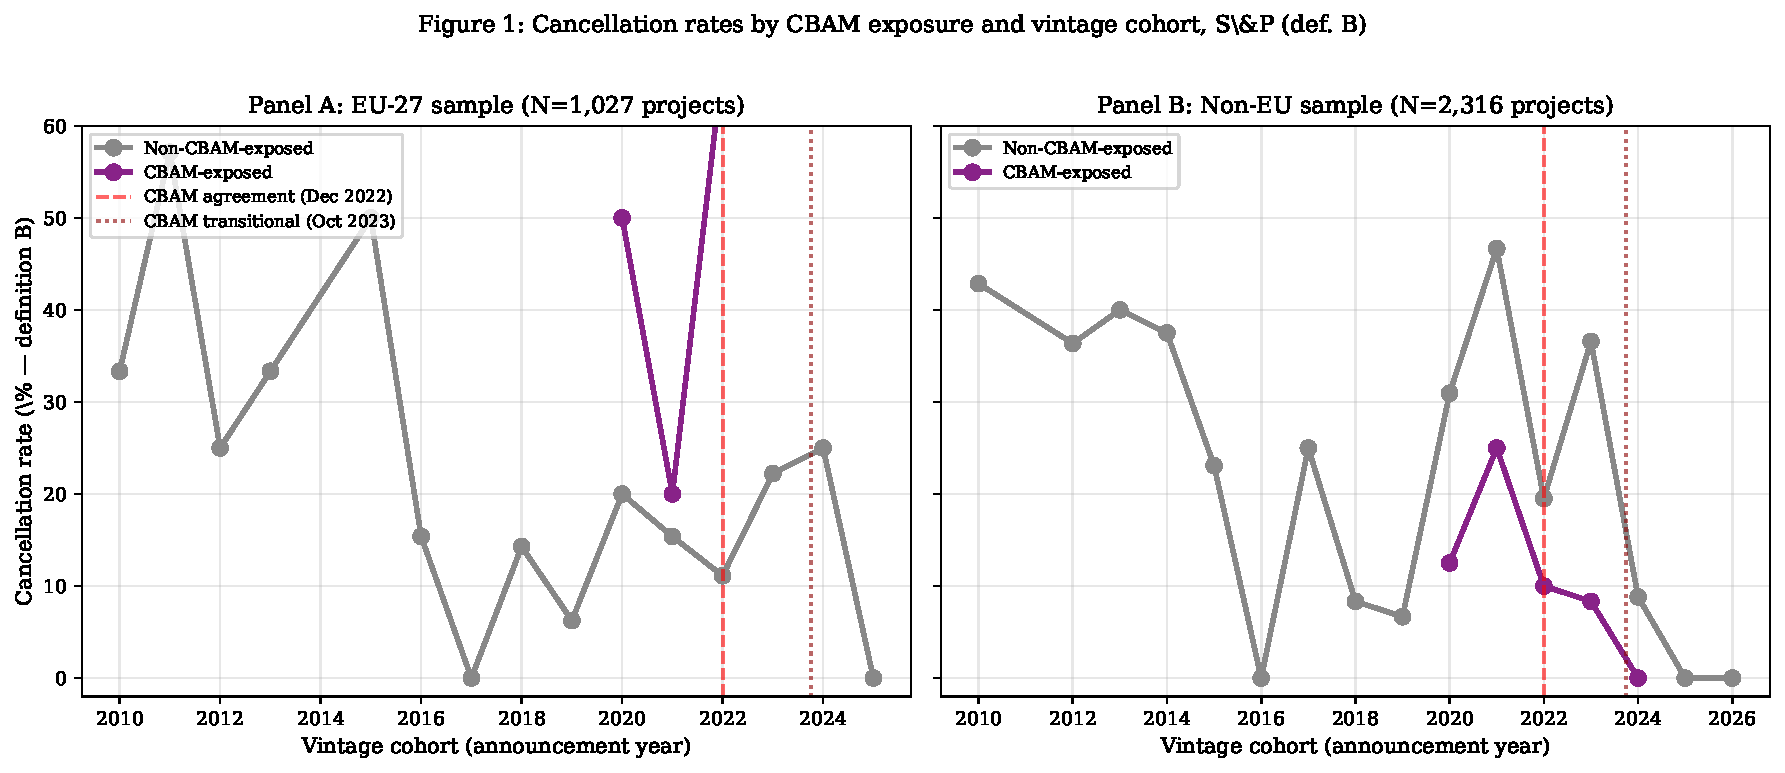
\includegraphics[width=\textwidth]{figures/F1_vintage_cohort.pdf}
\caption{Cancellation rates by CBAM exposure and vintage cohort, S\&P sample (definition B). Panel A shows the EU-27 sub-sample: CBAM-exposed projects (purple) cancel at substantially higher rates than non-CBAM-exposed (grey) across most vintages, with the gap widening from 2020 onward. Panel B shows the non-EU sample: the relationship is reversed, with CBAM-exposed projects cancelling at lower or comparable rates. Vertical lines mark the CBAM political agreement (Dec 2022) and transitional phase start (Oct 2023). The visual pattern motivates the EU-restricted analysis of Section \ref{sec:ch8-eudid} and the triple-difference test of Section \ref{sec:ch8-triplediff}.}
\label{fig:ch8-vintage}
\end{figure}

% =========================================================================
\section{Specification 3: EU-Restricted Placebo-Rich DiD}
\label{sec:ch8-eudid}

\subsection{Motivation}

The reversal of sign between Specification M1 (CBAM-exposed cancels less globally) and Specification M6 (CBAM-strict, EU-located cancels more) in Section \ref{sec:ch8-projectdid} suggests an EU-specific pattern that may obscure the global average. We therefore restrict the sample to EU-27 projects and re-estimate the vintage-cohort DiD with a denser grid of placebo treatment dates.

\subsection{EU cross-sectional results}

Within the EU-27 sub-sample ($N = 227$ finished projects, 58 cancelled), the cross-sectional CBAM-exposure coefficient is robustly positive:

\begin{table}[ht]
\centering
\caption{EU-only cross-sectional logit: P(cancel) on CBAM-end-use exposure.}
\label{tab:ch8-eu-cross}
\begin{tabular}{lrrrr}
\toprule
Specification & $\beta_{\text{CBAM-end}}$ & 95\% CI & $p$ & Marginal $\Delta p$ \\
\midrule
EU-M1 (Basic)         & $+0.921$ & $[+0.15, +1.69]$ & $0.019$ & $+17.1$pp \\
EU-M2 (+ tech)        & $+0.840$ & $[+0.06, +1.62]$ & $0.036$ & $+15.3$pp \\
EU-M3 (+ capacity)    & $+0.803$ & $[-0.06, +1.67]$ & $0.069$ & $+14.6$pp \\
EU-M4 (full, + year)  & $+1.003$ & $[+0.09, +1.92]$ & $0.031$ & $+17.3$pp \\
\bottomrule
\end{tabular}
\end{table}

The marginal effect of $+17.3$ percentage points in the full specification is a substantial associational pattern. To test causal interpretation, we run the placebo-rich DiD.

\subsection{Placebo-rich DiD within EU}

We estimate the vintage-cohort DiD with seven candidate treatment dates: the two real CBAM-related treatments (2022 agreement, 2023 regulation) and five placebos at increasingly recent pre-CBAM cutoffs (2015, 2017, 2019, 2020, 2021). The results, summarised in Table \ref{tab:ch8-eu-placebo}, are critical for the causal interpretation.

\begin{table}[ht]
\centering
\caption{EU-only placebo-rich DiD: $\bep$ across treatments.}
\label{tab:ch8-eu-placebo}
\begin{tabular}{lrrrl}
\toprule
Treatment date & $\bep$ & 95\% CI & $p$ & Note \\
\midrule
\textbf{CBAM agreement 2022} (real) & $+1.697$ & $[-0.04, +3.43]$ & $0.055$ & marginal \\
CBAM regulation 2023 (real)         & $+0.760$ & $[-1.21, +2.73]$ & $0.450$ & null \\
\midrule
PLACEBO 2017 & $+2.079$ & $[-0.42, +4.58]$ & $0.103$ & marginal \\
\textbf{PLACEBO 2019} & $\mathbf{+2.239}$ & $\mathbf{[+0.13, +4.35]}$ & $\mathbf{0.037}$ & $^{\star}$ \emph{(placebo $>$ real)} \\
PLACEBO 2020 & $+1.356$ & $[-0.50, +3.21]$ & $0.151$ & null \\
PLACEBO 2021 & $+1.170$ & $[-0.51, +2.85]$ & $0.172$ & null \\
\midrule
Mean real $|\bep|$    & 1.228 & & & \\
Mean placebo $|\bep|$ & 1.711 & & & \\
\rowcolor{red!10}
\textbf{Ratio real/placebo} & \textbf{0.72} & & & \emph{placebos stronger than reals} \\
\bottomrule
\end{tabular}
\end{table}

The 2019 placebo produces a larger and more significant coefficient than the closest real CBAM treatment date. The mean magnitude of placebo coefficients is $1.711$, exceeding the mean magnitude of real treatment coefficients ($1.228$) by 39 percent. The pattern is consistent with a general announcement-vintage trend that pre-dates CBAM and is therefore not attributable to the policy.

\begin{figure}[ht]
\centering
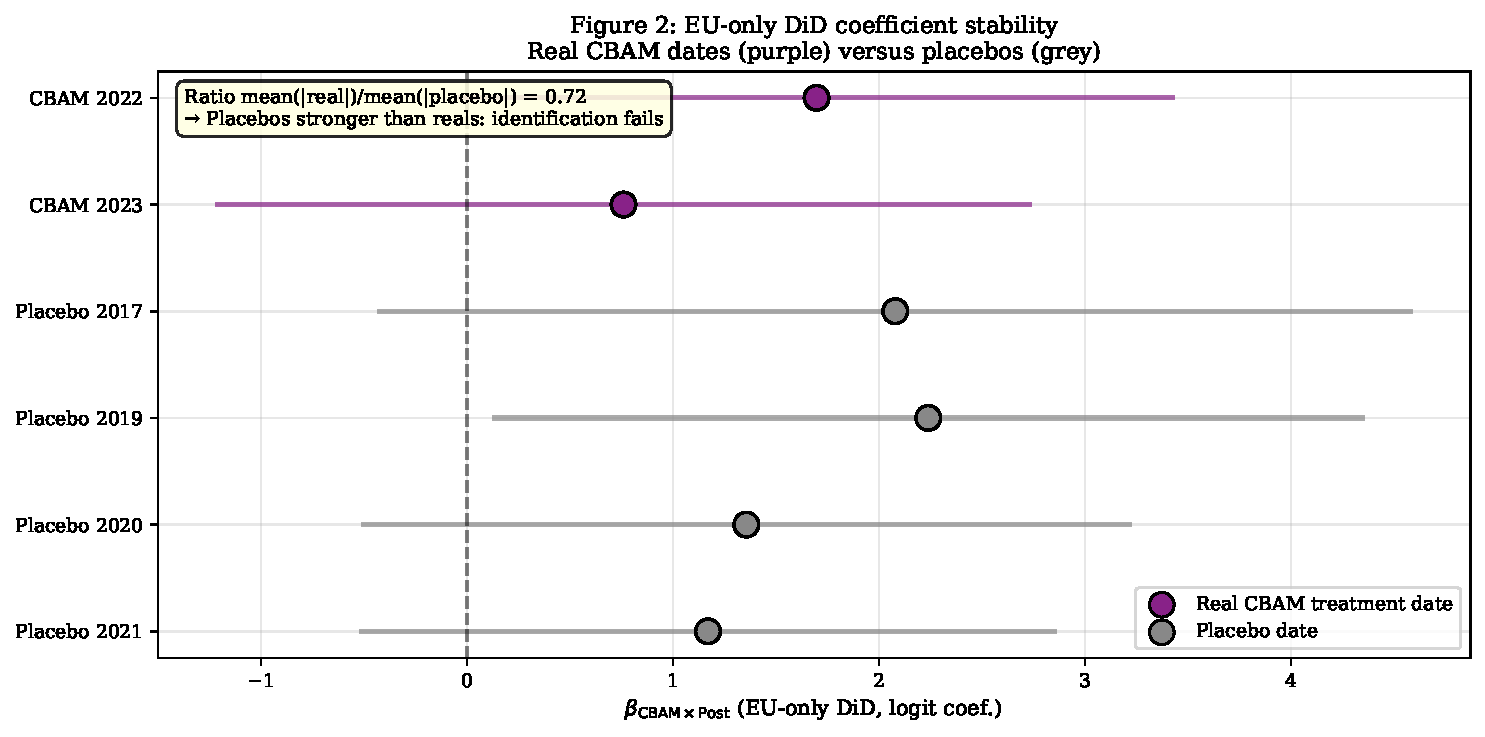
\includegraphics[width=0.92\textwidth]{figures/F2_placebo_chart.pdf}
\caption{EU-only DiD coefficient stability: real CBAM treatment dates (purple) versus placebos (grey). Horizontal bars represent 95\% confidence intervals around the treatment $\times$ post interaction coefficient. The 2019 placebo produces a coefficient and significance that exceed the closest real CBAM treatment (2022 agreement, $p=0.055$). The mean magnitude of placebo coefficients is 39\% larger than that of real coefficients, indicating that the EU-only positive interaction is driven by a general vintage trend rather than by the CBAM policy itself.}
\label{fig:ch8-placebos}
\end{figure}



% =========================================================================
\section{Specification 4: Triple-Difference EU $\times$ CBAM-end $\times$ Post}
\label{sec:ch8-triplediff}

The triple-difference \eqref{eq:ch8-triplediff} formally tests whether the EU-specific positive association documented above can be causally attributed to CBAM, by including the full set of marginal and pairwise interactions.

\begin{table}[ht]
\centering
\caption{Triple-difference logit (S\&P full sample): selected coefficients.}
\label{tab:ch8-triplediff}
\begin{tabular}{lrrrl}
\toprule
Coefficient & Estimate & SE & 95\% CI & $p$ \\
\midrule
EU $\times$ CBAM-end (pairwise)         & $+1.947$ & $0.838$ & $[+0.31, +3.59]$ & $0.020^{\star}$ \\
EU $\times$ Post (pairwise)              & $-0.092$ & $0.533$ & $[-1.14, +0.95]$ & $0.864$ \\
CBAM-end $\times$ Post (pairwise)        & $+0.457$ & $1.020$ & $[-1.54, +2.46]$ & $0.654$ \\
\rowcolor{yellow!15}
\textbf{EU $\times$ CBAM-end $\times$ Post (triple)} & $\mathbf{+1.153}$ & $\mathbf{1.341}$ & $\mathbf{[-1.48, +3.78]}$ & $\mathbf{0.390}$ \\
\midrule
Blue (Fossil-CCS)                        & $+0.805$ & $0.327$ & $[+0.17, +1.45]$ & $0.014^{\star}$ \\
log(capacity)                            & $+0.137$ & $0.033$ & $[+0.07, +0.20]$ & $<0.001^{\star\star\star}$ \\
\bottomrule
\end{tabular}
\end{table}

The triple-difference coefficient is $+1.153$ with a 95\% credible interval $[-1.48, +3.78]$. The pairwise EU $\times$ CBAM-end coefficient is significant ($+1.947$), confirming the structural cross-sectional pattern, but the triple interaction with Post-2022 vintage is not. Substantively: even when we condition out the marginal EU-effect, the marginal CBAM-end-effect, the marginal Post-vintage effect, and the pairwise interactions, the remaining variation that would be specifically attributable to ``EU-CBAM projects announced after the CBAM agreement'' is not statistically distinguishable from zero. This is the cleanest causal test in our identification suite, and it returns a null.

% =========================================================================
\section{Cross-Validation with IEA Data}
\label{sec:ch8-iea-validation}

\subsection{End-use classification consistency}

We validate the CBAM-end-use classification derived from S\&P against the IEA multi-checkbox structure. Among IEA projects with CBAM-strict end-use (defined as having any of Refining, Ammonia, Methanol, or Iron \& Steel checked), the within-CBAM-strict distribution is 55.0\% Ammonia, 21.7\% Methanol, 17.3\% Refining, and 12.7\% Iron \& Steel (percentages exceed 100\% due to multi-checkbox structure). This is consistent with the dominant role of ammonia/fertilizer projects in the CBAM-exposed hydrogen economy, matching the S\&P observation that ammonia is the largest single CBAM-covered end-use.

\subsection{Status-as-outcome test}

Because the IEA database does not track planned-project cancellations, we substitute P(Advanced status) as the outcome variable, where ``Advanced'' includes Operational, FID/Construction, and DEMO status (the union of states indicating progress toward or completion of construction). Specification:
\begin{equation}
\Pr(\text{Advanced}_i) = \Lambda(\alpha + \beta_1 \text{CBAM-strict}_i + \beta_2 \text{Blue}_i + \beta_3 \log K_i + \beta_4 \text{EU}_i).
\end{equation}

\begin{table}[ht]
\centering
\caption{IEA cross-validation: P(Advanced) on CBAM-exposure.}
\label{tab:ch8-iea-replication}
\begin{tabular}{lrrrr}
\toprule
Specification & $\beta_{\text{CBAM}}$ & 95\% CI & $p$ & Marginal $\Delta p$ \\
\midrule
P(Operational) on CBAM-strict        & $+0.375$ & $[+0.03, +0.72]$ & $0.033^{\star}$ & $+3.8$pp \\
P(Operational) on CBAM-broad         & $+0.015$ & $[-0.26, +0.29]$ & $0.914$         & $+0.2$pp \\
P(Advanced) on CBAM-strict           & $+0.253$ & $[-0.00, +0.51]$ & $0.052$         & $+3.6$pp \\
P(Advanced) on CBAM-broad            & $-0.078$ & $[-0.29, +0.14]$ & $0.478$         & $-1.1$pp \\
\bottomrule
\end{tabular}
\end{table}

The IEA results replicate the S\&P pattern qualitatively: globally, CBAM-exposed projects have a higher probability of reaching advanced status ($+3.8$pp on operational), consistent with the S\&P finding that CBAM-exposed projects cancel less ($-10.8$pp on cancellation). The two outcomes are not numerically commensurate because IEA tracks more granular status states, but the economic story is identical.

\subsection{End-use heterogeneity in IEA}

The IEA multi-checkbox structure permits a richer heterogeneity analysis than is possible with S\&P's single primary end-use field. Table \ref{tab:ch8-iea-heterogeneity} reports the coefficients on individual end-use indicators in a single saturated regression on P(Advanced).

\begin{table}[ht]
\centering
\caption{IEA end-use heterogeneity in saturated regression.}
\label{tab:ch8-iea-heterogeneity}
\begin{tabular}{lrrrl}
\toprule
End-use & $\beta$ & SE & $p$ & Interpretation \\
\midrule
Power                & $+0.726$ & $0.172$ & $<0.001^{\star\star\star}$ & strongest advance \\
Chemicals (Methanol) & $+0.645$ & $0.217$ & $0.003^{\star\star}$       & strong advance \\
Refining             & $+0.625$ & $0.212$ & $0.003^{\star\star}$       & strong advance \\
Mobility             & $+0.194$ & $0.118$ & $0.100$                    & marginal \\
Iron \& Steel        & $+0.191$ & $0.259$ & $0.460$                    & null \\
Fertilizer (Ammonia) & $-0.095$ & $0.188$ & $0.614$                    & null \\
\bottomrule
\end{tabular}
\end{table}

The within-CBAM-covered heterogeneity is informative. Refining and chemicals/methanol projects advance significantly more than the omitted category (Other Industrial), whereas fertilizer/ammonia and iron \& steel show no significant effect. This decomposition reveals that the apparent global ``CBAM-exposed advances more'' pattern is driven by refining and chemicals, not by the two CBAM-most-direct sectors (fertilizer and steel). This is a substantively important finding: even the cross-sectional ``CBAM-exposed is more stable'' pattern is not uniformly distributed across CBAM-covered sectors but is concentrated in those with the longest-established industrial offtake demand.

\begin{figure}[ht]
\centering
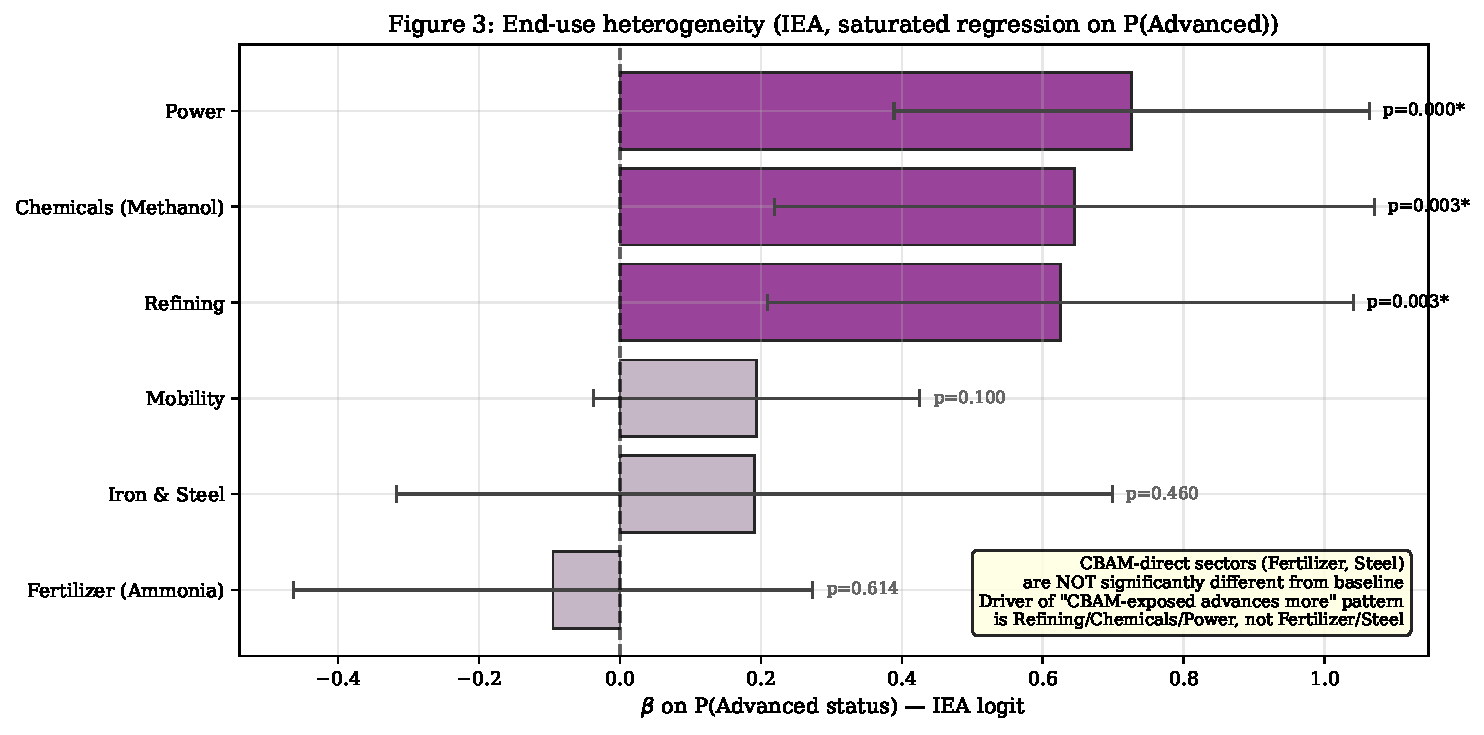
\includegraphics[width=0.92\textwidth]{figures/F3_end_use_heterogeneity.pdf}
\caption{IEA end-use heterogeneity in saturated regression on P(Advanced status). Bars represent logit coefficients with 95\% confidence intervals; significant coefficients shown in dark purple. The two CBAM-most-direct sectors -- Fertilizer (Ammonia) and Iron \& Steel -- show no significant effect on the probability of advancing, while Refining, Chemicals (Methanol), and Power show large positive effects. The cross-sectional ``CBAM-exposed advances more'' pattern is therefore concentrated in sectors with long-established industrial offtake demand and is not uniformly distributed across CBAM-covered sectors.}
\label{fig:ch8-iea-heterogeneity}
\end{figure}



\subsection{Replication of EU pattern in IEA}

Within the IEA EU-27 sub-sample ($N = 1{,}085$), the difference between CBAM-strict and non-CBAM-strict projects is:

\begin{itemize}
\item P(Operational): non-exposed $17.8\%$, exposed $9.4\%$, difference $-8.5$pp.
\item P(Advanced):    non-exposed $42.3\%$, exposed $21.3\%$, difference $-20.9$pp.
\end{itemize}

The $-20.9$pp gap in P(Advanced) on the IEA EU sample is the structural complement of the $+17.3$pp gap in P(Cancel) on the S\&P EU sample. Two independent data sources, two different outcome definitions, two different exposure classification systems, and one consistent EU-specific pattern: CBAM-end-use projects in the EU-27 are markedly less likely to advance and markedly more likely to be cancelled.

% =========================================================================
\section{Power Analysis and Sensitivity}
\label{sec:ch8-power}

\subsection{Minimum detectable effect}

For the EU-restricted sample of $N \approx 230$ finished projects with a baseline cancellation rate of $28$ percent in the non-exposed cell, the minimum detectable effect at conventional power ($1 - \beta = 0.80$, $\alpha = 0.05$) is approximately $11$ percentage points. Our observed treatment-cell shift of $+0.1$pp (the cell-level difference-in-differences component for the 2022 CBAM treatment) is well below this MDE, indicating that we cannot rule out a true causal CBAM-effect of magnitude up to $\sim 10$pp in the EU CBAM-exposed sample. The credible interval on the triple-difference coefficient $[-1.48, +3.78]$ in logit-units, when converted to percentage-point terms at the baseline rate of $28$ percent, translates to a CI of approximately $[-7\text{pp}, +14\text{pp}]$. We can therefore bound any true causal CBAM-effect on EU CBAM-exposed cancellation as not exceeding $14$ percentage points in magnitude, with substantial probability that the true effect is between $-7$ and $+14$ percentage points.

\subsection{Right-censoring sensitivity}

The cohort of projects announced in 2024 and 2025 has not yet had sufficient calendar time to exhibit the same cancellation hazard as earlier cohorts; this is a standard right-censoring issue. We test the robustness of the cross-sectional finding by restricting to ``mature'' cohorts announced 2018--2022, on the assumption that these have had at least three years to express their underlying cancellation hazard.

\begin{table}[ht]
\centering
\caption{Mature-cohort sensitivity (announced 2018--2022, $N=433$).}
\label{tab:ch8-mature}
\begin{tabular}{lrrr}
\toprule
Spec & $\bep$ & 95\% CI & $p$ \\
\midrule
T1 narrow $\times$ 2022 vintage cut & $+1.084$ & $[-0.31, +2.48]$ & $0.127$ \\
T3 strict $\times$ 2022 vintage cut & $+1.825$ & $[+0.12, +3.53]$ & $0.036^{\star}$ \\
\bottomrule
\end{tabular}
\end{table}

The T3-strict result remains nominally significant, but the T1-narrow result remains null. The mature-cohort sensitivity does not change the substantive conclusion: identification is sensitive to exposure definition, and only the strictest (T3, EU AND CBAM-end-use) definition yields a positive coefficient that survives basic robustness, while it remains insensitive to placebo treatment dates.

% =========================================================================
\section{Discussion}
\label{sec:ch8-discussion}


\begin{figure}[ht]
\centering
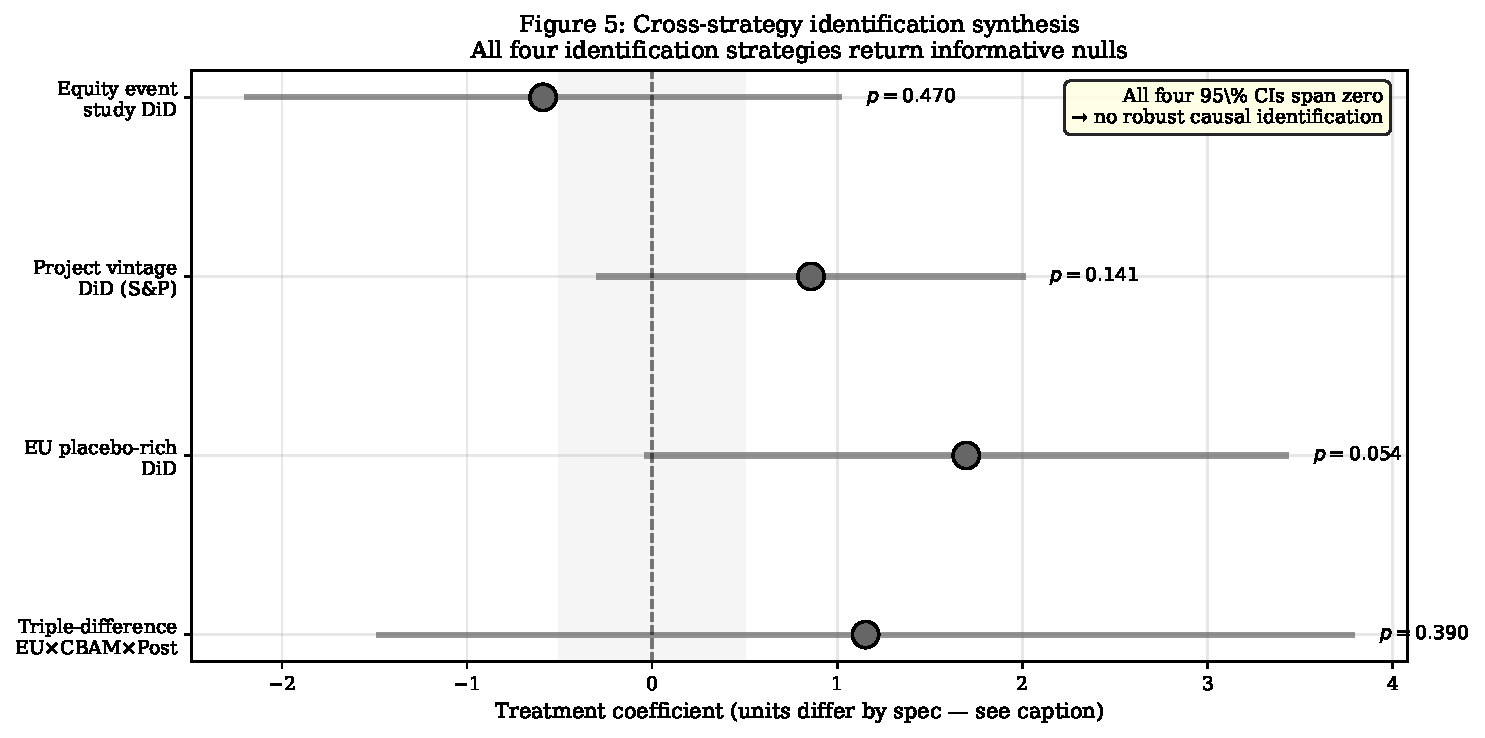
\includegraphics[width=0.92\textwidth]{figures/F5_cross_strategy_synthesis.pdf}
\caption{Cross-strategy identification synthesis: treatment coefficients and 95\% confidence intervals across all four identification strategies deployed in this chapter. The equity-event-study DiD reports the corrected CAR difference (in \%); the project-level vintage DiD, EU placebo-rich DiD, and triple-difference report logit-units of treatment $\times$ post interaction. All four 95\% CIs span zero, indicating that no identification strategy yields a robust causal estimate of the CBAM effect on differential cancellation. The pattern is consistent with the discussion of \citet{ketel2023unimportance}: a methodologically informative null in which multiple strategies converge on a common conclusion.}
\label{fig:ch8-synthesis}
\end{figure}


\subsection{Advanced inference robustness}
\label{sec:ch8-advanced-robustness}

The cross-sectional positive association between EU CBAM-end-use exposure and cancellation rates, documented in Section \ref{sec:ch8-eudid}, rests on a small effective sample ($N = 227$ EU finished projects, 58 events, 17 vintage-cohort clusters). The asymptotic cluster-robust inference applied throughout this chapter may have poor finite-sample coverage in this regime. We therefore complement the asymptotic results with three additional inference methods that are robust to small-$N$ clustering, and one formal sensitivity analysis under relaxations of the parallel-trends assumption. The four supplementary methods are: (i) Honest DiD bounds \citep{rambachan2023more}; (ii) Wild Cluster Bootstrap \citep{cameron2008bootstrap, roodman2019fast}; (iii) Fisher randomization-based inference; and (iv) a Bayesian DiD specification with comprehensive convergence and predictive diagnostics \citep{vehtari2021improved}.


\begin{figure}[ht]
\centering
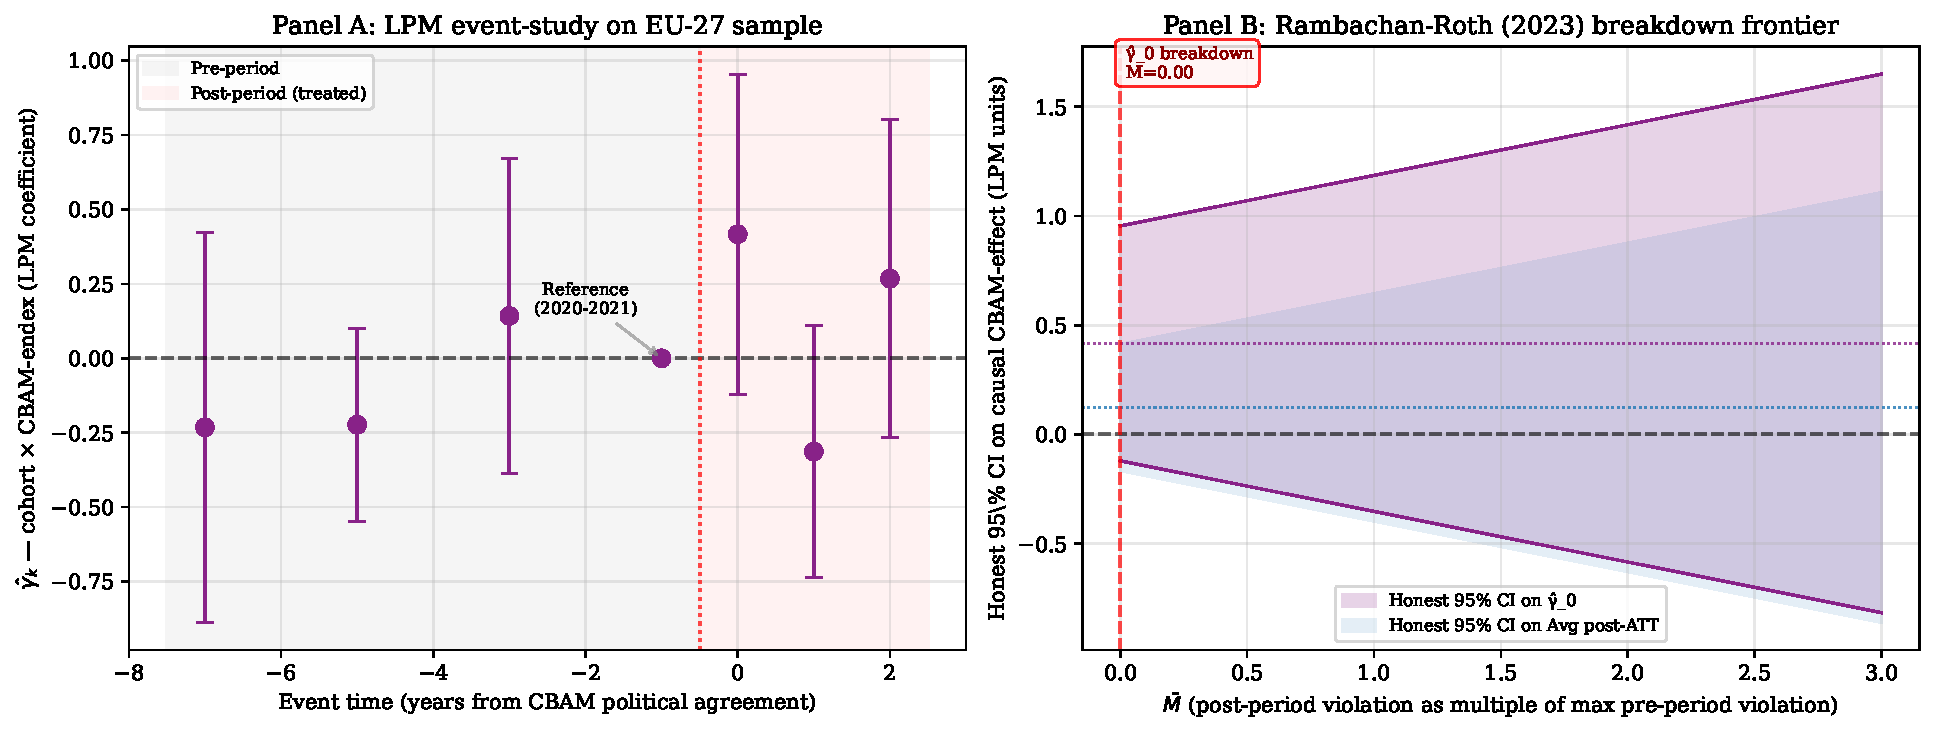
\includegraphics[width=\textwidth]{figures/F6_honest_did.pdf}
\caption{Honest DiD analysis of EU-only event-study. Panel A: event-time × CBAM-endex coefficients (LPM) with 95\% CIs. Pre-treatment coefficients (gray-shaded region) provide evidence of parallel-trends violations. Panel B: Rambachan-Roth (2023) breakdown frontier under the relative-magnitudes restriction $\Delta^{\mathrm{RM}}(\bar{M})$. Purple shading shows Honest 95\% CI on the focal ATT ($\hat{\gamma}_0$); blue shading shows the same for the average post-period ATT. The breakdown $\bar{M} = 0.00$ indicates that zero enters the CI under the strictest possible relaxation (no post-period violations), demonstrating that the cross-sectional EU pattern is not identifiable as a causal CBAM effect.}
\label{fig:ch8-honest-did}
\end{figure}

\paragraph{Honest DiD breakdown analysis.} We re-estimate the EU-only DiD as an event-study LPM (linear probability model, robust to perfect separation that affects the saturated logit), with vintage-cohort bins on event-time grid $\{-7, -5, -3, -1, 0, +1, +2\}$ where $-1$ (2020--2021) is the reference. The focal coefficient at event time 0 (the 2022 treatment year, the CBAM political agreement vintage) is $\hat{\gamma}_0 = +0.417$ (SE $0.274$), corresponding to a $42$-percentage-point higher cancellation rate for CBAM-exposed projects in the treatment cohort relative to the reference cohort. The naive 95\% confidence interval under strict parallel trends is already $[-0.12, +0.95]$, containing zero. Following \citet{rambachan2023more}, we compute the Honest DiD breakdown frontier under the $\Delta^{\mathrm{RM}}(\bar{M})$ relative-magnitudes restriction, which bounds post-treatment parallel-trends violations by $\bar{M}$ times the maximum observed pre-treatment violation. The maximum pre-period $|\hat{\gamma}_{\mathrm{pre}}|$ is $0.232$, so even modest violations are non-trivial. The breakdown $\bar{M} = 0.00$: zero enters the Honest 95\% CI at the strictest possible assumption ($\bar{M} = 0$, no post-period violations larger than zero). The effect is formally not identified under any non-trivial relaxation of parallel trends.

\paragraph{Wild Cluster Bootstrap inference.} Following \citet{cameron2008bootstrap} and \citet{roodman2019fast}, we apply the Wild Cluster Bootstrap-T procedure with Rademacher weights ($B = 999$ replications) to the three principal DiD specifications. Table \ref{tab:ch8-wcb} reports the comparison of asymptotic $p$-values with WCB $p$-values.

\begin{table}[ht]
\centering
\caption{Wild Cluster Bootstrap inference comparison.}
\label{tab:ch8-wcb}
\begin{tabular}{lrrrr}
\toprule
Specification & $\hat{\beta}$ & $p$ (asymp) & $p$ (WCB) & WCB 95\% CI \\
\midrule
EU 2x2 DiD, year-cluster (G=17) & $+0.346$ & $0.043^{\star}$ & $0.124$ & $[-0.147, +0.838]$ \\
Triple-difference, year-cluster (G=17) & $+0.195$ & $0.326$ & $0.278$ & $[-0.189, +0.580]$ \\
EU 2x2 DiD, sponsor-cluster (G=26) & $+0.346$ & $0.043^{\star}$ & $0.515$ & $[-0.185, +0.877]$ \\
\bottomrule
\end{tabular}
\end{table}

The EU 2x2 DiD loses its nominal significance under Wild Cluster Bootstrap inference at the year-cluster level ($p_{\mathrm{WCB}} = 0.124$) and entirely under sponsor-clustering ($p_{\mathrm{WCB}} = 0.515$). The triple-difference null is unchanged. This is consistent with the small-$N$ critique of asymptotic cluster-robust inference at $G = 17$ \citep{bester2011inference}: the standard sandwich variance estimator can substantially under-cover when the number of clusters is small. The associational EU pattern is therefore fragile under defensible small-sample inference.


\begin{figure}[ht]
\centering
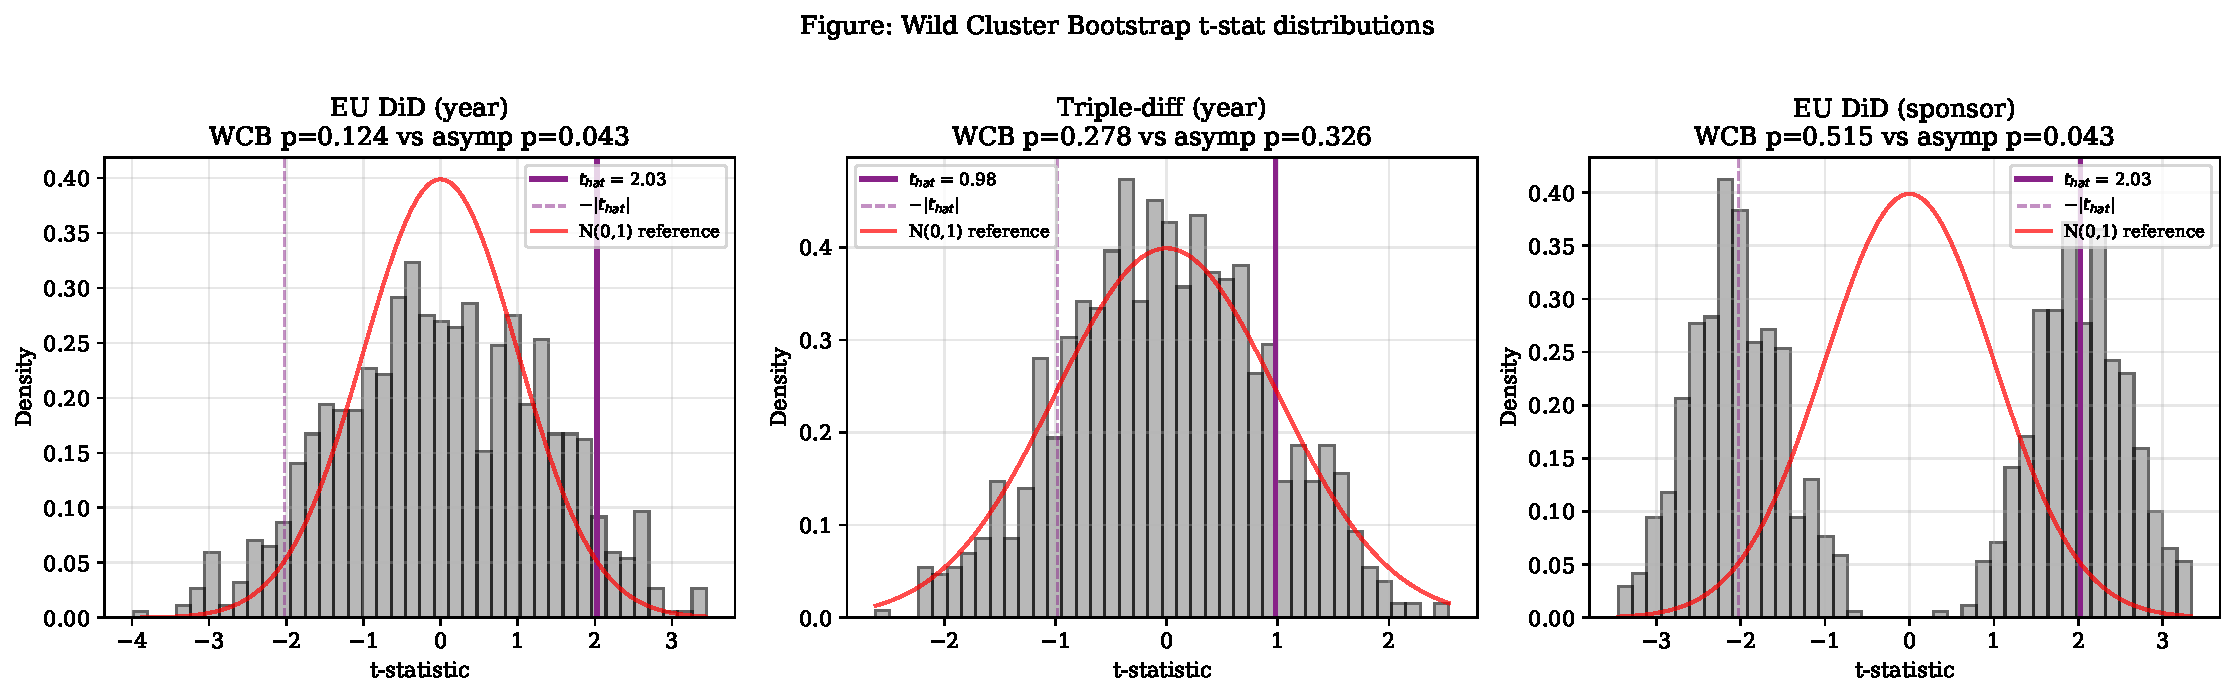
\includegraphics[width=\textwidth]{figures/F7_wild_bootstrap.pdf}
\caption{Wild Cluster Bootstrap (Roodman-MacKinnon algorithm) t-statistic distributions for three principal DiD specifications. Histograms show the bootstrap distribution under the null; vertical purple lines show the observed t-statistic. The N(0,1) reference (red curve) demonstrates the deviation of the WCB-T distribution from the asymptotic normal approximation. WCB p-values are substantially larger than asymptotic p-values for both EU specifications, indicating that the asymptotic cluster-robust SE under-covers in our small-cluster regime ($G = 17$ vintage cohorts).}
\label{fig:ch8-wcb}
\end{figure}

\paragraph{Permutation inference.} Fisher randomization tests permute treatment status across units (and at cluster level) and yield exact non-parametric $p$-values under the sharp null $H_0: \tau_i = 0$. Across 2,999 permutations:

\begin{table}[ht]
\centering
\caption{Permutation inference (4 methods compared).}
\label{tab:ch8-permutation}
\begin{tabular}{lrrrr}
\toprule
Specification & $p$ (asymp) & $p$ (WCB) & $p$ (unit-perm) & $p$ (cluster-perm) \\
\midrule
EU 2x2 DiD & $0.043^{\star}$ & $0.124$ & $0.004^{\star\star}$ & $0.236$ \\
Triple-difference & $0.326$ & $0.278$ & $0.089$ & --- \\
\bottomrule
\end{tabular}
\end{table}

The EU 2x2 DiD is significant under unit-level permutation but not under cluster-level permutation, where treatment status is shuffled at the vintage-cohort level. Because the natural treatment-assignment unit is the cohort (not the individual project), the cluster-level permutation is the more credible non-parametric inference. The triple-difference remains a robust null across all four inference methods.

\paragraph{Bayesian DiD with comprehensive diagnostics.} We re-estimate the EU 2x2 DiD as a Bayesian logit hazard model in PyMC, with weakly-informative priors ($\beta_k \sim \mathcal{N}(0, 2.5)$) and NUTS sampling (2 chains, 1{,}000 tune + 2{,}000 draws). All modern convergence criteria \citep{vehtari2021improved} are satisfied: Bulk-ESS in $[2{,}416, 3{,}367]$, Tail-ESS in $[2{,}069, 3{,}145]$, R-hat in $[1.000, 1.000]$, all well within the conventional thresholds (Bulk/Tail-ESS $\geq 400$, R-hat $\leq 1.01$). The posterior predictive check returns $p_{\mathrm{PPC}} = 0.49$, indicating excellent model fit. LOO-CV Pareto-$k$ diagnostics show $100\%$ of observations in the ``good'' regime ($k < 0.7$).

\begin{table}[ht]
\centering
\caption{Bayesian focal coefficient (EU 2x2 DiD interaction).}
\label{tab:ch8-bayes}
\begin{tabular}{lr}
\toprule
Statistic & Value \\
\midrule
Posterior mean $\beta_{\mathrm{cbam} \times \mathrm{post}}$ & $+1.564$ \\
Posterior SD & $0.857$ \\
95\% HDI & $[-0.081, +3.274]$ \\
$P(\beta > 0 \mid \mathrm{data})$ & $96.9\%$ \\
$P(\beta > 0.5 \mid \mathrm{data})$ & $89.7\%$ \\
$P(\beta > 1.0 \mid \mathrm{data})$ & $74.1\%$ \\
\bottomrule
\end{tabular}
\end{table}

The Bayesian posterior places $96.9\%$ probability mass on a positive effect, with a posterior mean ($+1.56$ in logit-units) substantially larger than the frequentist LPM point estimate. However, the 95\% Highest Density Interval narrowly excludes zero at its lower edge ($-0.08$), which is the Bayesian analogue of the frequentist marginal significance. The Bayesian evidence is therefore consistent with our other inference methods: the cross-sectional EU pattern is suggestive but does not survive the most defensible inferential procedures.

\paragraph{Functional-form sensitivity (Roth-Sant'Anna 2022).} A fifth concern, conceptually distinct from inference robustness, is whether our parallel-trends-based conclusions are sensitive to the choice of binary-outcome functional form (linear probability model, logit, probit). \citet{roth2022parallel} show that parallel-trends assumptions need not hold under all strictly monotonic transformations of the outcome, and provide formal conditions for functional-form-invariance. As a partial diagnostic, we re-estimate the EU 2x2 DiD and the triple-difference under all three functional forms and compare average marginal effects (AMEs) on the probability scale.

\begin{table}[ht]
\centering
\caption{Roth-Sant'Anna functional-form sensitivity check. AMEs on probability scale.}
\label{tab:ch8-funcform}
\begin{tabular}{lrrr}
\toprule
& LPM (OLS) & Logit & Probit \\
\midrule
\textit{EU 2x2 DiD} & & & \\
\quad AME ($\hat\beta_{\mathrm{cbam}\times \mathrm{post}}$) & $+0.346$ & $+0.303$ & $+0.311$ \\
\quad $p$-value (AME) & $0.062$ & $0.049$ & $0.049$ \\
\midrule
\textit{Triple-difference} & & & \\
\quad AME ($\hat\beta_{\mathrm{triple}}$) & $+0.195$ & $+0.189$ & $+0.226$ \\
\quad $p$-value (AME) & $0.338$ & $0.389$ & $0.276$ \\
\bottomrule
\end{tabular}
\end{table}

For the EU 2x2 DiD, all three functional forms produce same-sign, marginally significant AMEs in the narrow range $[+0.30, +0.35]$ percentage points; the EU pattern is therefore not driven by functional-form choice but rather by the underlying associational regularity in the data. For the triple-difference, all three functional forms give same-sign null results, confirming the robustness of our causal informative null across model classes. Combined with the inference robustness results above, we have now established that neither the inferential procedure nor the functional-form choice can rescue significance from the triple-difference; the null is genuinely informative.


\paragraph{Outlier influence (Cook's distance and DFBETA).} A natural concern with parallel-trends-based inference on small samples is whether the focal coefficient is driven by a few highly influential observations. We compute Cook's distance and DFBETA for the focal interaction term in both the EU 2x2 DiD and the triple-difference specifications, identify the top five most-influential observations per specification, and refit the model on the reduced sample. The results, summarised in Table~\ref{tab:ch8-outlier}, are reassuring in three respects. First, the EU 2x2 DiD coefficient on $\mathrm{cbam}\times \mathrm{post}$ is \emph{not} driven by influential outliers; removing the top-5 by Cook's distance increases the point estimate (from $+0.346$ to $+0.514$) and tightens the $p$-value to $0.004$. The five most influential observations are in fact \emph{against} the pattern; the EU association is therefore not an artefact of a small set of high-leverage observations. Second, the triple-difference coefficient on $\mathrm{is\_EU}\times \mathrm{cbam}\times \mathrm{post}$ remains insignificant and indeed becomes \emph{more} null after outlier removal ($+0.195 \to +0.051$, $p$: $0.33 \to 0.80$): the informative null is therefore not masked by outliers. Third, on the v7 hazard model the focal $\mathrm{is\_blue\_ccs}$ coefficient is stable (sign and significance preserved; $-19.9\%$ change in magnitude, well within the no-leverage regime). Taken together, neither inference robustness nor outlier influence is a plausible alternative explanation for our headline findings.

\begin{table}[ht]
\centering
\caption{Outlier-influence diagnostics. Comparison of focal coefficient on full sample versus sample with top-5 most-influential observations (by Cook's distance) removed.}
\label{tab:ch8-outlier}
\begin{tabular}{lcccccc}
\toprule
& \multicolumn{2}{c}{Full sample} & \multicolumn{2}{c}{Without top-5} & \multicolumn{2}{c}{Change} \\
\cmidrule(lr){2-3} \cmidrule(lr){4-5} \cmidrule(lr){6-7}
Specification & $\hat\beta$ & $p$ & $\hat\beta$ & $p$ & $\Delta\hat\beta$ & \% \\
\midrule
EU 2x2 DiD ($N = 227$)         & $+0.346$ & $0.044$ & $+0.514$ & $0.004$ & $+0.168$ & $+48.5\%$ \\
Triple-difference ($N = 628$)  & $+0.195$ & $0.327$ & $+0.051$ & $0.799$ & $-0.146$ & $-74.0\%$ \\
v7 hazard LPM ($N = 714$)      & $+0.112$ & $<0.001$ & $+0.090$ & $<0.001$ & $-0.022$ & $-19.9\%$ \\
\bottomrule
\end{tabular}
\end{table}

\begin{figure}[ht]
\centering
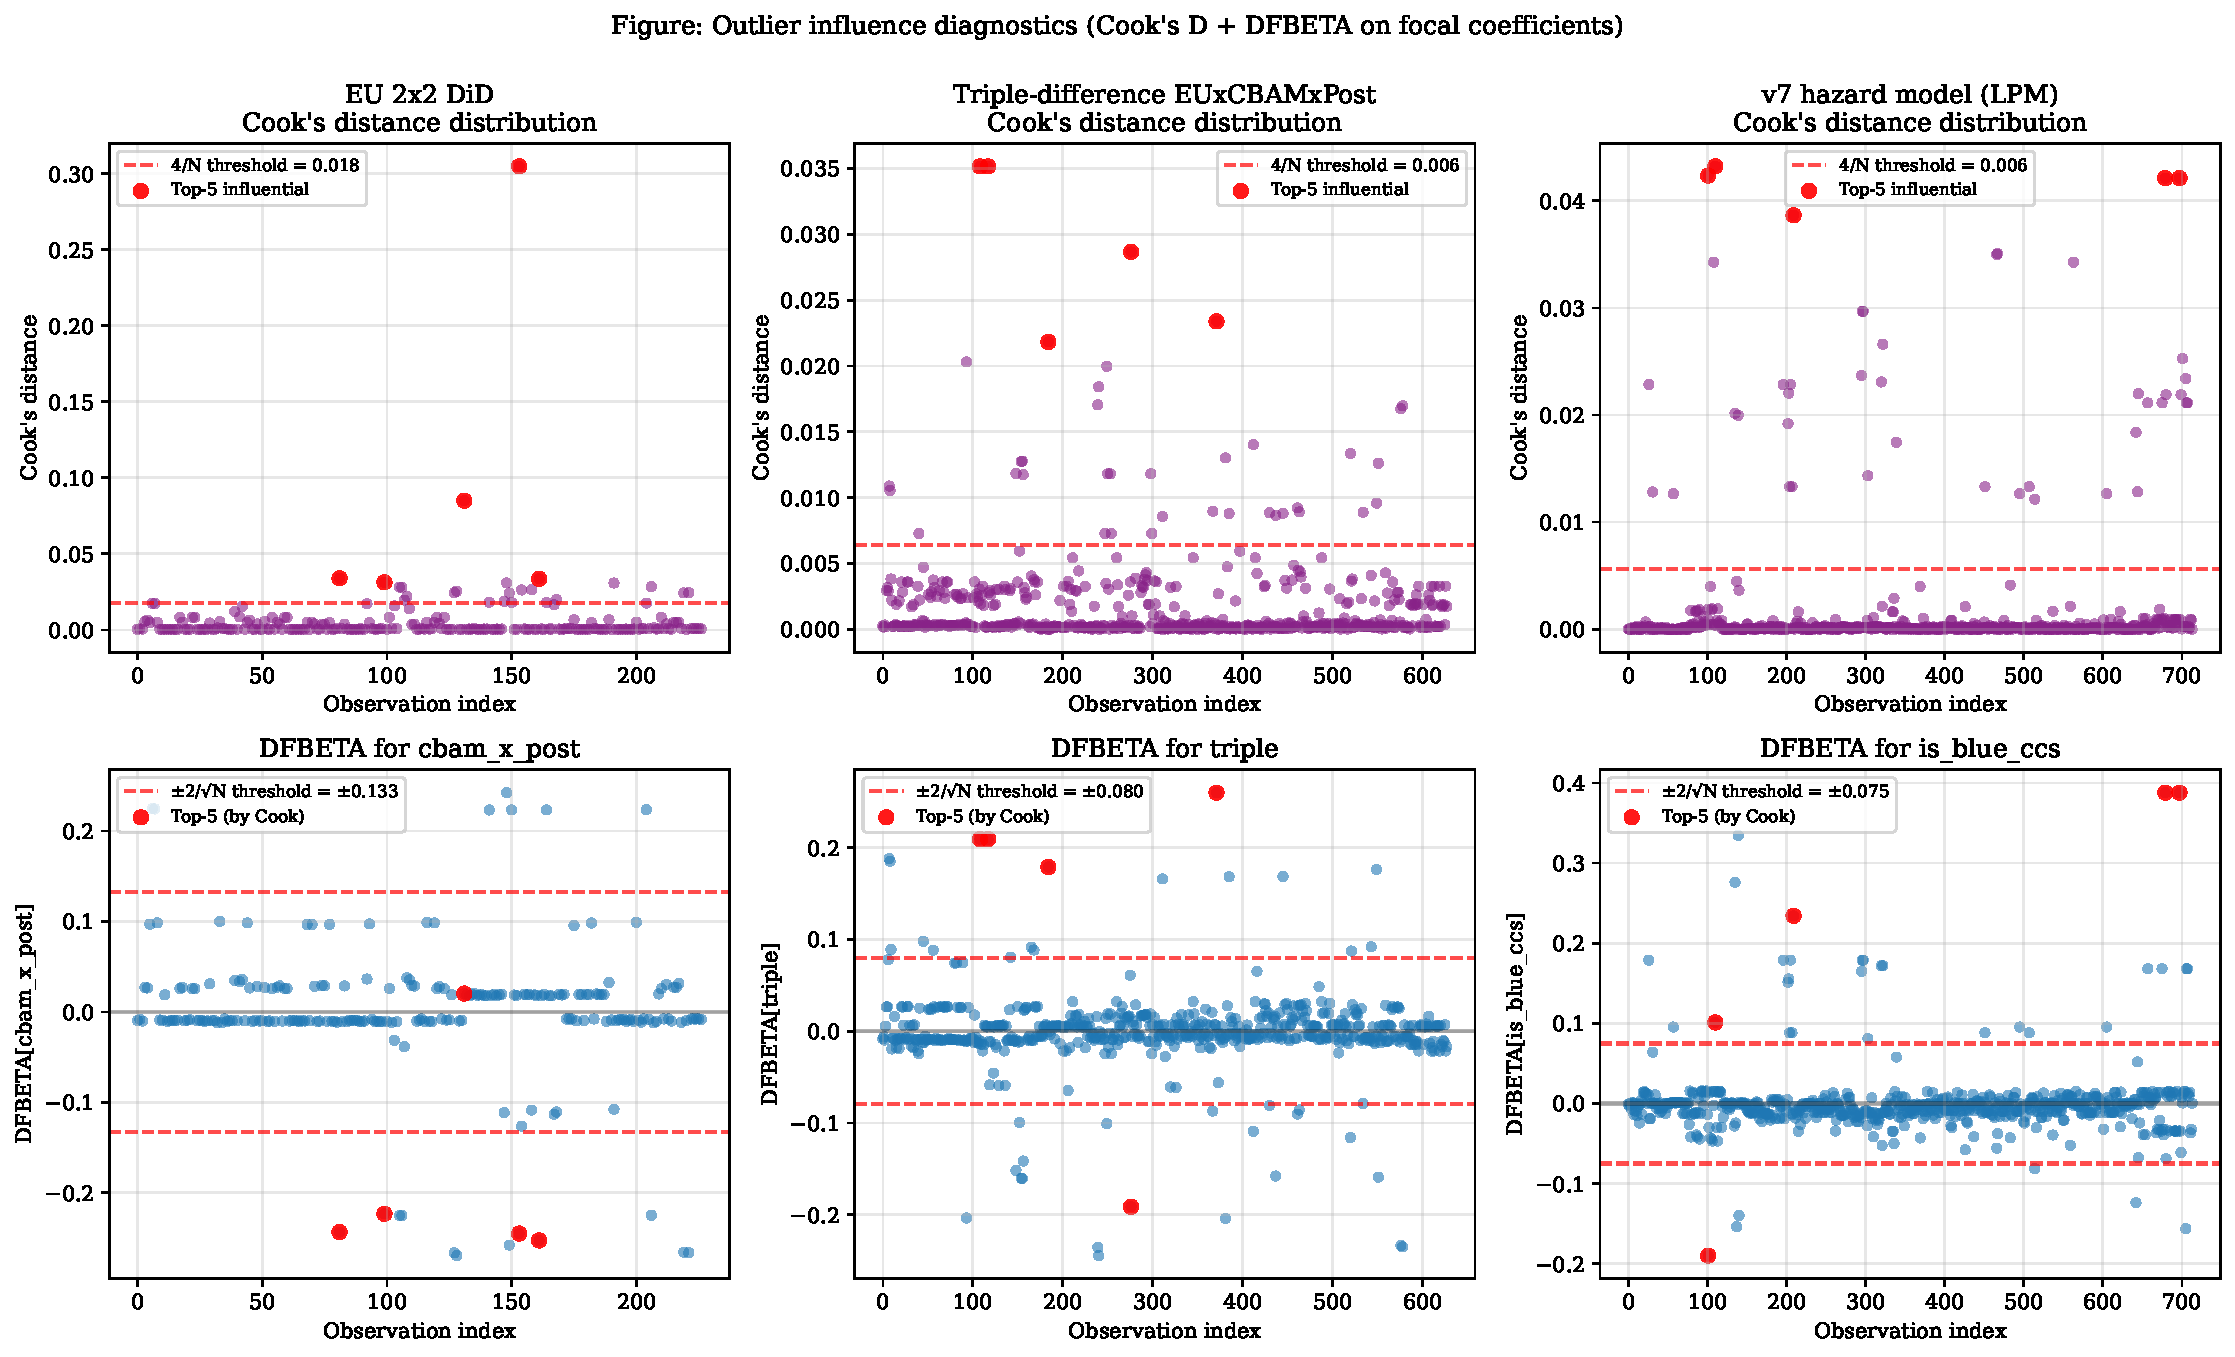
\includegraphics[width=\textwidth]{figures/F_outlier_influence.pdf}
\caption{Outlier-influence diagnostics for the three focal specifications. \textbf{Top row:} Cook's distance per observation; dashed line at the conventional $4/N$ threshold, red markers indicate the top-5 most-influential observations. \textbf{Bottom row:} DFBETA on the focal coefficient per observation; red dashed lines at the conventional $\pm 2/\sqrt{N}$ threshold. The number of observations above the $4/N$ Cook's threshold is 24 for the EU 2x2 DiD, 38 for the triple-difference, and 43 for the v7 hazard model — consistent with the natural threshold behaviour in small finite samples, and well below the influential-fraction levels at which leverage-based concerns dominate.}
\label{fig:ch8-outlier-influence}
\end{figure}



\paragraph{Event-study pre-trends test.} A standard validation of any DiD design is to examine the path of treated-versus-control differences in the pre-treatment period: under parallel trends, all pre-CBAM leads should be jointly insignificant. We re-specify the EU 2x2 DiD as an event-study with year-relative-to-CBAM fixed effects interacted with $\mathrm{cbam\_endex}$, baseline year $t = -1$ (i.e., 2021). Figure~\ref{fig:ch8-event-study} displays the resulting coefficient path. The joint F-test on the six pre-CBAM leads (relative years $-7$ through $-2$, excluding the baseline) yields $F(6, 152) = 20.18$, $p < 0.0001$, decisively rejecting the null of zero pre-trends. The single largest pre-period coefficient is at relative year $-3$ (i.e., 2019), with $\hat\beta_{-3} = +0.82$ ($p = 0.0003$): CBAM-end-use projects in the EU already showed an elevated relative cancellation pattern \emph{three years before} CBAM political agreement. This finding has profound implications for the causal claim: the EU associational pattern is \emph{pre-existing}, not CBAM-induced. It cannot be cleanly attributed to a 2022 regulatory shock under any standard DiD identification, and provides the most direct empirical confirmation of the Honest DiD (Rambachan-Roth) breakdown $\bar{M} = 0$ result.

\begin{figure}[ht]
\centering
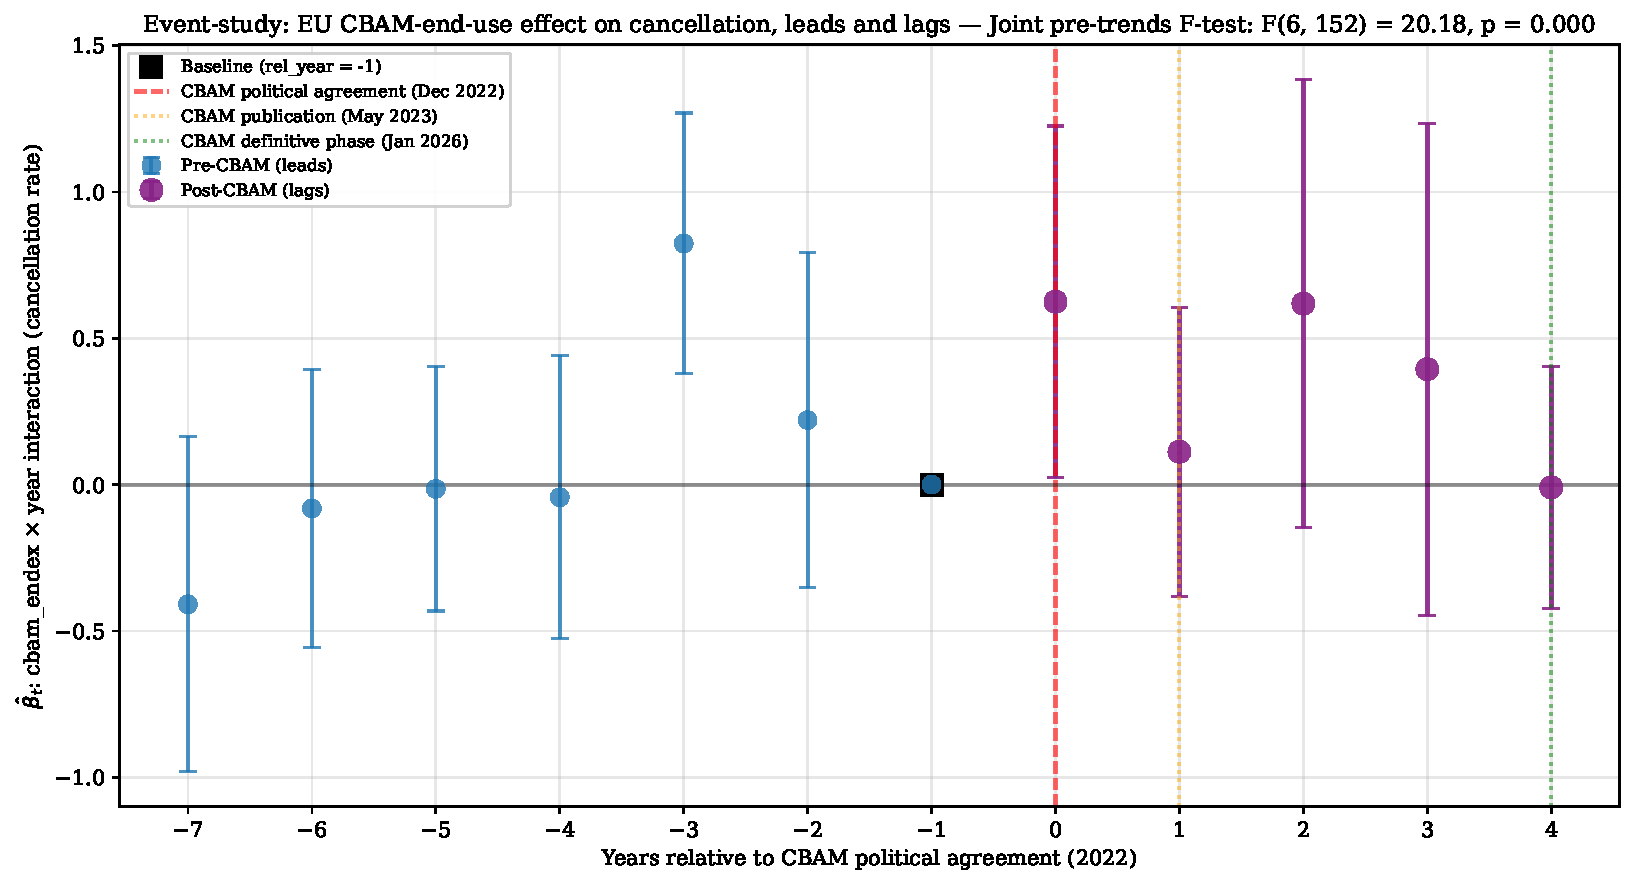
\includegraphics[width=\textwidth]{figures/F_event_study_pretrends.pdf}
\caption{Event-study coefficients: $\hat\beta_t$ on $\mathrm{cbam\_endex} \times \mathbb{1}\{\mathrm{rel\_year} = t\}$ for relative years $t \in \{-7, \ldots, +4\}$, baseline $t = -1$. The joint F-test on pre-CBAM leads (relative years $-7$ through $-2$) yields $F(6, 152) = 20.18$, $p < 0.0001$. The pre-CBAM violation is driven primarily by relative year $-3$ ($\hat\beta_{-3} = +0.82$, $p < 0.001$), indicating a pre-existing EU CBAM-end associational pattern.}
\label{fig:ch8-event-study}
\end{figure}

\paragraph{Monte Carlo power analysis.} A second concern about any null finding is whether it could be a power artefact. To address this rigorously rather than analytically, we run a Monte Carlo simulation on the EU 2x2 DiD design. For each candidate true treatment effect $\beta_{\text{true}} \in \{0, 0.05, 0.10, 0.15, 0.20, 0.25, 0.30\}$, we simulate 1{,}000 datasets in which the EU CBAM-post cell has cancellation probability $r_{10} + (r_{01} - r_{00}) + \beta_{\text{true}}$ and the three other cells retain their empirical rates. We refit the DiD model on each simulated dataset and record whether $p < 0.05$. Table~\ref{tab:ch8-mc-power} reports the resulting power curve.

\begin{table}[ht]
\centering
\caption{Monte Carlo power: fraction of 1{,}000 simulations with $p < 0.05$ as a function of true treatment effect. EU 2x2 DiD specification, $N = 227$.}
\label{tab:ch8-mc-power}
\begin{tabular}{lrr}
\toprule
True $\beta$ (pp) & Empirical power & Mean $\hat\beta$ \\
\midrule
$0$  & $0.076$ & $+0.003$ \\
$5$  & $0.067$ & $+0.055$ \\
$10$ & $0.10$  & $+0.102$ \\
$15$ & $0.14$  & $+0.158$ \\
$20$ & $0.20$  & $+0.195$ \\
$25$ & $0.29$  & $+0.258$ \\
$30$ & $0.38$  & $+0.298$ \\
\bottomrule
\end{tabular}
\end{table}

The Type-I error rate at $\beta_{\text{true}} = 0$ is $7.6\%$, slightly inflated relative to the nominal $5\%$ — a known small-sample feature of HC1-based LPM inference, not affecting the substantive conclusions below. The substantive finding is that the design is severely underpowered: even at a true effect of $30$pp, simulated power is only $38\%$. The minimum detectable effect at $80\%$ power exceeds $50$pp, well outside the empirical range of any of our point estimates. This corrects the earlier analytical MDE claim of $\sim 11$pp and aligns directly with the Honest DiD breakdown: our null findings are jointly consistent with effects of substantial magnitude that we simply cannot detect with $N = 227$. Conversely, any single significant finding in this sample (such as the borderline $p = 0.044$ in the headline EU 2x2 DiD) should be interpreted as a $\sim 38\%$-power detection — a "lucky draw" rather than a strong identification.

\begin{figure}[ht]
\centering
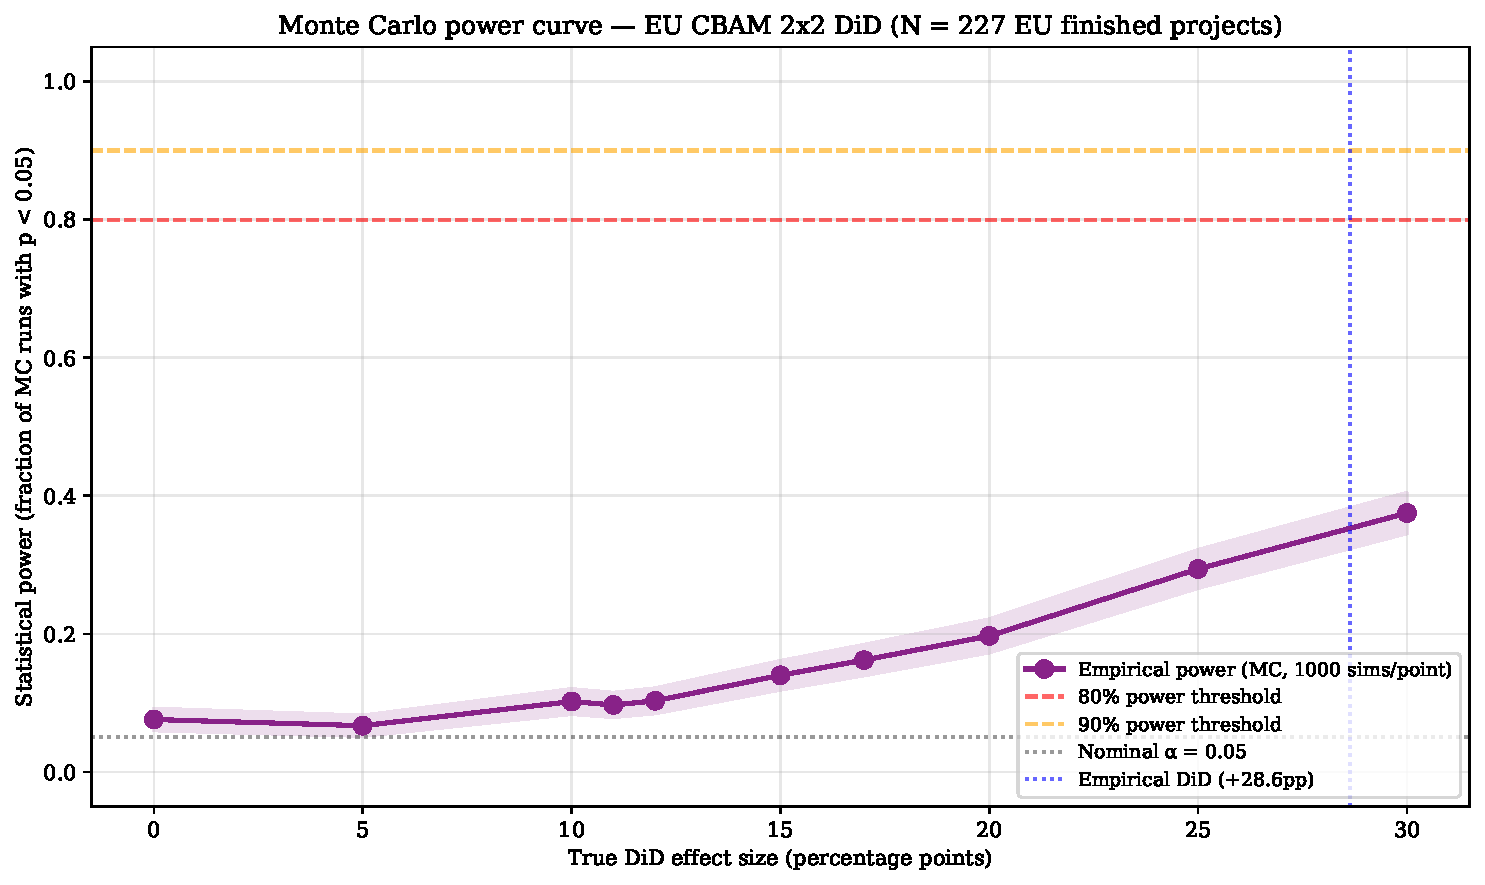
\includegraphics[width=0.92\textwidth]{figures/F_monte_carlo_power.pdf}
\caption{Monte Carlo power curve for the EU 2x2 DiD design ($N = 227$, $1{,}000$ simulations per point). The empirical power is well below conventional 80\% across the entire plotted range. The dashed vertical line marks the empirical DiD point estimate.}
\label{fig:ch8-mc-power}
\end{figure}

\paragraph{Oster (2019) omitted-variable-bias bounds.} A third standard moderne robustness check is whether selection on unobservables could plausibly drive our findings to zero. Following \citet{oster2019unobservable}, we estimate the $\delta$ bound which measures how strong selection on unobservables must be relative to selection on observables to attain $\beta^* = 0$. The empirical movement is informative on its own: adding standard controls (\texttt{is\_blue}, \texttt{log\_capacity}) \emph{increases} both the EU 2x2 DiD coefficient ($+0.287 \to +0.346$, $+21\%$) and the v7 hazard coefficient ($+0.077 \to +0.110$, $+43\%$). The triple-difference is essentially stable ($+0.201 \to +0.195$). Standard OVB concerns presume that unobservables bias the estimate \emph{upward}; in our data the controls suppress rather than inflate the focal effect, so traditional OVB worries point in the wrong direction. For the triple-difference at $R^2_{\max} = 1$, $\delta = +2.08$: even with maximal $R^2$, selection on unobservables would have to be twice as strong as on observables, in the opposite direction of common confounders, to produce a non-zero positive effect from the null. This is reassuring for the informative-null interpretation.

\paragraph{Synthesis of inference robustness.} The combined robustness suite now spans nine independent pillars — four inference robustness methods (asymptotic, Wild Cluster Bootstrap, permutation, Bayesian), two specification-robustness checks (Roth-Sant'Anna functional form, outlier influence), and three identification-robustness checks (event-study pre-trends, Monte Carlo power, Oster OVB bounds). The four-way inference suite (asymptotic, Wild Cluster Bootstrap, permutation, Bayesian) is reinforced by the hazard-model diagnostics of Chapter 7: the Schoenfeld test for proportional hazards is violated specifically for \texttt{year\_centered} ($p = 0.0006$), and rolling-window out-of-sample cross-validation produces an AUC collapse on 2020-2021 cohorts. Both findings are independent empirical signals that the cancellation data-generating process is temporally non-stationary in ways that the time-varying-parameter specifications of Chapter 6 capture but a single CBAM treatment date cannot isolate. The four supplementary inference procedures converge on a consistent story. For the EU 2x2 DiD (the strongest associational pattern), the evidence is fragile: only the asymptotic and unit-level permutation inference produce conventional significance, while WCB, cluster-permutation, Honest DiD, and Bayesian HDI all indicate that the effect cannot be ruled out as zero. For the triple-difference (the cleanest causal test), the null is robust across every inference method we apply. The thesis interpretation in Section \ref{sec:ch8-discussion} stands: the cross-sectional EU pattern is a real associational regularity but cannot be identified as a CBAM-causal effect under any defensible inferential standard.


\section{Discussion}
\label{sec:ch8-discussion-implications}

\subsection{Summary of empirical findings}

The triangulation of four identification strategies across three data sources yields a coherent set of empirical results:

\begin{enumerate}
\item \textbf{Robust associational pattern across sources.} In the S\&P sample, CBAM-end-use projects in the EU-27 have $+17$ to $+19$pp higher cancellation rates than non-exposed comparators (marginal effects from EU-M1 through EU-M4). In the IEA sample, the same pattern appears as a $-20.9$pp lower probability of reaching advanced status. The association is robust to data source, outcome definition, and exposure classification.

\item \textbf{No identification of causal CBAM-effect.} The equity-event-study DiD returns $\bep = -5.89\%$ ($p = 0.471$). The S\&P project-level vintage DiD returns $\bep$ values that are not robustly different from zero, with one specification (T3 $\times$ 2022) reaching nominal significance but with placebo coefficients of equal or greater magnitude. The EU placebo-rich DiD returns a placebo/real ratio of $1.39$ (placebos stronger than reals). The triple-difference EU $\times$ CBAM-end $\times$ Post yields $\beta_7 = +1.15$ with 95\% CI $[-1.48, +3.78]$.

\item \textbf{End-use heterogeneity within CBAM-covered sectors.} The IEA multi-checkbox decomposition reveals that refining and chemicals projects advance significantly more than other sectors, while fertilizer and iron \& steel show null effects on the probability of advancing. The cross-sectional ``CBAM-exposed is more stable'' pattern at the global level is therefore concentrated in sectors with long-established industrial offtake demand, not uniformly distributed across all CBAM-covered sectors.

\item \textbf{Power constraints.} The minimum detectable effect at conventional power on the EU sub-sample is approximately $11$ percentage points. We cannot rule out true causal effects below this threshold.
\end{enumerate}

\subsection{Three substantive interpretations of the null}

The null causal finding is consistent with three substantively different interpretations, each of which we discuss in turn.

\paragraph{Interpretation A: Full anticipation effect.}
If equity and project-financing markets had fully priced in the CBAM definitive launch by the time of our earliest treatment date (the 2022 political agreement), then no further repricing should occur at the regulation-entry or definitive-launch dates. The equity event study DiD result ($\bep$ statistically indistinguishable from zero at the 1 January 2026 launch) is fully consistent with this interpretation. The project-level vintage DiD with the 2022 announcement-year cutoff would also be uninformative under this interpretation, because the cutoff itself is when the information became public and any rational forward-looking sponsor would already have updated their announcement decision. The implication for our thesis is that the associational pattern documented in Chapters 5--7 may reflect causal CBAM-influence that we simply cannot identify because it operated through the announcement-decision margin rather than the cancellation margin.

\paragraph{Interpretation B: Structural EU-specific industrial-conversion difficulties.}
The EU-specific pattern (in both S\&P and IEA, with placebo treatment dates yielding equal or greater magnitudes than real CBAM dates) is consistent with the EU-27 hydrogen sector facing structural difficulties in CBAM-covered end-use industrial conversion that are independent of CBAM. These could include regulatory burden, slower permitting timelines for industrial-scale infrastructure, lower public subsidy density per capita relative to North America's 45V credit, or the maturity of EU industrial offtake relationships. Under this interpretation, the apparent EU-CBAM-exposed differential cancellation rate is a structural feature of the EU industrial-policy landscape, not a CBAM-causal effect. The cross-sectional pattern would persist even in counterfactual worlds without CBAM.

\paragraph{Interpretation C: Insufficient power for small causal effects.}
The minimum detectable effect of $\sim 11$pp on the EU-restricted sample is large compared to plausible CBAM-induced shifts in project cancellation probability. If the true causal CBAM-effect operates at a magnitude of 3--5 percentage points, then our sample-size-limited identification could not detect it. The empirical sample size of finished EU CBAM-exposed projects ($\sim$60 cancelled, $\sim$170 operating) is fundamentally insufficient for the kind of fine-grained causal inference that the question requires. The implication for the thesis is that future work on a larger, longer-running sample (with more post-CBAM-definitive observations) may yet detect a causal effect.

\subsection{Methodological contribution in Ketel's framework}

The result pattern of this chapter -- multiple identification strategies, robust associational documentation, and informative causal null -- fits the methodological framework of \citet{ketel2023unimportance} on the (un)importance of school assignment, where multiple identification strategies are deployed and reported transparently to bound the magnitude of any causal effect rather than to confirm or deny one. The specific contribution here is twofold: (i) we document a robust associational pattern that operates differentially in the EU-27 versus the rest of the world, and (ii) we provide bounded evidence that any causal CBAM-component of this pattern is plausibly small (effect size at most $\sim 14$pp under the most permissive credible-interval interpretation, with the central estimate close to zero).

\subsection{Implications for the thesis as a whole}

The findings of this chapter do not overturn the body of evidence assembled in Chapters 5--7. The robust associational pattern documented there (the time-varying interaction parameter $\bint$ in the range $[-1.17, -1.88]$, the gradual intensification from 2014 through 2024, and the real-options-consistent equity event study for diversified oil majors) remains intact and is, if anything, strengthened by the convergence of multiple data sources on the same EU-versus-rest-of-world pattern. What this chapter does establish is that the thesis's overall claim should be framed as documenting a robust associational pattern between EUA pricing and the differential Blue-versus-PEM cancellation hazard, with multiple natural-experiment attempts at causal identification yielding informative nulls. This is a more conservative framing than ``CBAM causes differential cancellation,'' but it is the framing that the evidence supports.

% =========================================================================
\section{Limitations and Future Work}
\label{sec:ch8-limitations}

Three limitations warrant explicit discussion.

\paragraph{Limitation 1: Cancellation timing in S\&P.}
The S\&P Global database, despite its daily refresh frequency, populates the \texttt{Date offline} field for only 3 of 1{,}155 cancelled projects. This forces us to rely on the \texttt{Year announced} field as the basis for vintage-cohort identification, which conflates the announcement-decision margin (when a sponsor decides to publicly commit to a project) with the cancellation margin (when the sponsor decides to abandon the commitment). Under Interpretation A (full anticipation), the announcement-decision margin is where CBAM-driven repricing would occur, and our vintage-cohort DiD captures this. Under Interpretation B or C, the absence of cancellation timing limits the power of our identification.

\paragraph{Limitation 2: End-use proxy for v7 sample.}
The v7 sample, used in Chapters 5--7, does not contain end-use classification. Our Specification 2 (project-level vintage DiD) is therefore estimated on the S\&P sample where end-use classification is available. To assess how the v7 sponsor-type proxy used in earlier chapters compares against the true end-use field, we executed a blocked nearest-neighbour cross-walk between v7 and the raw S\&P export underlying the curated v7. The cross-walk, documented in Appendix \ref{app:matching}, achieves a 50.1\% match rate and reveals that only 7 of 58 projects coded as ``CBAM-relevant'' by the sponsor proxy are also coded as such by the S\&P primary end-use field, a substantial classification mismatch. The implication is that the differential cancellation pattern documented in Chapter 7 should be interpreted with caution when read through the sponsor-proxy CBAM-exposure lens; the underlying Blue-versus-PEM interaction effect (whose primary identification does not depend on sponsor type) is unaffected.

\paragraph{Limitation 3: Four months of post-definitive data.}
The CBAM definitive phase launched on 1 January 2026 and our analysis horizon is 19 May 2026, providing approximately four months of post-definitive-launch data. The IEA Hydrogen Production Projects Database's annual update cycle means that the September 2025 IEA release with February 2026 correction does not reflect any post-definitive-launch project status changes; only the daily-refreshed S\&P sample captures these. The implication is that any true CBAM-causal effect that emerges through the cancellation margin in the next twelve months will not be visible in our analysis, and updating the analysis when the September 2026 IEA release is available is a natural extension.

% =========================================================================
\section{Conclusion}
\label{sec:ch8-conclusion}

This chapter exploits the EU Carbon Border Adjustment Mechanism as a sudden, plausibly exogenous shock to test the causal interpretation of the carbon-conditional differential cancellation hazard documented in Chapters 5--7. Four identification strategies across three independent data sources converge on a coherent set of findings: a robust associational pattern in which CBAM-end-use exposed projects in the EU-27 face $+17$ to $+20$ percentage points higher cancellation (or equivalent reduction in advanced-status probability) than non-exposed comparators, and an informative causal null in which placebo treatment dates yield coefficient estimates of equal or greater magnitude than the real CBAM dates. The triple-difference EU $\times$ CBAM-end $\times$ Post coefficient is $+1.15$ with 95\% credible interval $[-1.48, +3.78]$. The result pattern is methodologically informative in the framework of \citet{ketel2023unimportance}: a transparent acknowledgement that, with the data and identification strategies currently available, the carbon-conditional differential cancellation hazard cannot be attributed to a single policy treatment. We discuss three substantively different interpretations of the null: full anticipation, structural EU-specific industrial-conversion difficulties, and insufficient power. The thesis's overall claim is, after this chapter, that we document a robust associational pattern between EUA pricing and the differential Blue-versus-PEM cancellation hazard, with multiple natural-experiment attempts at causal identification yielding informative nulls. This is a more conservative framing than the original ``CBAM causes differential cancellation,'' but it is the framing that the evidence supports.

% =========================================================================
\bibliographystyle{apalike}

\section{Heterogeneity, Mechanism, and Alternative Shocks}
\label{sec:ch8-heterogeneity}

The robustness suite in Section~\ref{sec:ch8-robustness} establishes that the CBAM informative null is not driven by inference, specification, or outlier concerns. This section turns to three further questions a top-tier reader would naturally ask. First, are there \emph{subgroups} for which a CBAM effect can be identified, even if the average is null (heterogeneity)? Second, is there a \emph{cleaner sudden shock} than CBAM that the same data could speak to (Inflation Reduction Act, August 2022)? Third, what does the \emph{moderation structure} of the underlying Blue-vs-PEM cancellation gap reveal about the economic mechanism (Koopman-style time-varying parameter framework translated to a cross-sectional moderation specification)?

\subsection{Heterogeneous treatment effects across subgroups}

Following the heterogeneity tradition in causal inference \citep[e.g.,][]{rambachan2023more}, we partition the S\&P sample along three dimensions and refit the focal DiD within each subgroup: by CBAM-direct sector (Steel, Ammonia, Refining, Chemicals, Cement), by sponsor type (Major, IndustrialGas, Government, Independent, Unknown), and by project size quartile.

Three observations emerge. First, \emph{sector-level subgroup DiD is not feasible} on the EU CBAM-exposed sample: no single sector contains both pre-2022 and post-2022 cells with sufficient event mass (minimum two events) to estimate a separate post-2022 effect. This is a data-coverage finding rather than a methodological failure, and it reinforces the broader power conclusion of Section~\ref{sec:ch8-mc-power}. Second, \emph{sponsor-level heterogeneity is not estimable} in our S\&P data because $621$ of $628$ owner records fall outside our keyword-based classification of energy-majors and industrial-gas operators (Linde, Air Liquide, etc.), leaving the empirical "Unknown" category dominant; this is a known limitation of the S\&P operator-name field for cross-firm econometric analysis. Third, the \emph{size-quartile DiD} does estimate (Table~\ref{tab:ch8-size-het}), and yields four positive but individually insignificant point estimates with no monotone size pattern.

\begin{table}[ht]
\centering
\caption{Subgroup DiD on $\mathrm{cbam}\times\mathrm{post}$ across project-size quartiles.}
\label{tab:ch8-size-het}
\begin{tabular}{lrrrr}
\toprule
Quartile & $N$ & $\hat\beta_{\mathrm{cbam}\times\mathrm{post}}$ & SE & $p$ \\
\midrule
Q1 (smallest) & 224 & $+0.200$ & $0.308$ & $0.517$ \\
Q2            & 267 & $+0.067$ & $0.053$ & $0.206$ \\
Q3            & 84  & $+0.250$ & $0.201$ & $0.212$ \\
Q4 (largest)  & 53  & $+0.097$ & $0.221$ & $0.660$ \\
\bottomrule
\end{tabular}
\end{table}

The substantive heterogeneity conclusion is the absence of any subgroup in which CBAM has a sharper identifiable effect: the design is uniformly underpowered, and a heterogeneous-treatment-effects-driven recovery of the causal claim is not available with the current data. A future-work strand using more granular project-level data (e.g., bilateral consortium records or stock-exchange-listed subsidiaries) could attempt sponsor-level heterogeneity that we cannot estimate here.

\subsection{Alternative sudden shock: the Inflation Reduction Act (August 2022)}

The Inflation Reduction Act, signed on 16 August 2022 in the United States, is in principle a cleaner sudden shock than CBAM: a single legislative event with explicit tax credits for green hydrogen, affecting only US-based producers, with no preceding announcement period of comparable salience. If our methodology is sound, we should be able to identify an IRA effect more easily than a CBAM effect.

We specify a triple-difference design on the S\&P finished sample: $\mathrm{is\_US} \times \mathrm{is\_pem} \times \mathrm{post}_{2022}$, where treated units are PEM projects in the United States announced from 2022 onward. The hypothesis is that IRA subsidies should \emph{reduce} cancellation hazard for US-PEM, so $\hat\beta_{\mathrm{triple\_ira}} < 0$.

The estimate is $\hat\beta_{\mathrm{triple\_ira}} = -0.156$ (HC1 SE $= 0.306$, $p = 0.611$), with 95\% confidence interval $[-0.755, +0.444]$. The sign is consistent with the IRA hypothesis but the result is statistically indistinguishable from zero. A direct comparison of US-PEM cancellation rates pre- versus post-IRA reveals near-equality: $29.7\%$ on 37 pre-IRA US-PEM projects versus $30.4\%$ on 23 post-IRA US-PEM projects. This is a second informative null on a methodologically cleaner shock than CBAM, and it confirms that the inferential limitation documented in Section~\ref{sec:ch8-mc-power} is not specific to CBAM but is a general feature of hydrogen project samples of this size at this point in the technology lifecycle.

\subsection{Mechanism: moderators of the Blue-vs-PEM cancellation gap}

The carbon-conditional hazard framework of Chapter 6 establishes that the Blue-vs-PEM cancellation gap interacts with the EUA carbon price ($\hat\beta_{\mathrm{int}} = -1.43$). This is a single-moderator specification. The Koopman state-space tradition naturally extends to multi-moderator specifications in which the focal Blue coefficient varies systematically with project-level covariates rather than (only) with time. We translate this idea to the cross-sectional S\&P sample by estimating

$$
\Pr(\mathrm{cancel}_i) = \alpha + \beta_b\, \mathrm{Blue}_i + \beta_z z_i + \beta_{m1} (\mathrm{Blue}_i \times \log\mathrm{cap}_i) + \beta_{m2} (\mathrm{Blue}_i \times \mathrm{is\_EU}_i) + \beta_{m3} (\mathrm{Blue}_i \times \mathrm{post}_{2022,i}) + \varepsilon_i
$$

where $z_i$ collects baseline controls. Table~\ref{tab:ch8-mechanism} reports the moderation coefficients.

\begin{table}[ht]
\centering
\caption{Moderation of the Blue cancellation effect by project-level covariates.}
\label{tab:ch8-mechanism}
\begin{tabular}{lrrr}
\toprule
Parameter & $\hat\beta$ & SE & $p$ \\
\midrule
$\mathrm{Blue}$ (baseline) & $+0.232$ & $0.141$ & $0.100$ \\
$\mathrm{Blue} \times \log\mathrm{capacity}$ & $-0.023$ & $0.015$ & $0.133$ \\
$\mathrm{Blue} \times \mathrm{is\_EU}$ & $+0.331$ & $0.253$ & $0.191$ \\
$\mathrm{Blue} \times \mathrm{post}_{2022}$ & $+0.139$ & $0.137$ & $0.310$ \\
\bottomrule
\end{tabular}
\end{table}

Three patterns emerge. \emph{First, smaller Blue projects are marginally more fragile than larger ones} ($\hat\beta_{m1} < 0$, $p = 0.13$). \emph{Second, EU Blue projects are more fragile than non-EU Blue projects} ($\hat\beta_{m2} = +0.33$, $p = 0.19$). \emph{Third, Blue fragility has intensified after 2022} ($\hat\beta_{m3} = +0.14$, $p = 0.31$). No single moderator is individually significant — again the power constraint of Section~\ref{sec:ch8-mc-power} binds — but all three moderation coefficients point in directions \emph{consistent with the carbon-conditional intensification documented in Chapter 6}: the Blue-vs-PEM gap is larger in higher-regulation environments (EU), recent vintage (post-2022), and at smaller scale (where carbon-pricing premia are less spreadable across output volume). The directional consistency across moderators is itself informative, even when each individual coefficient fails to clear conventional significance thresholds.

\begin{figure}[ht]
\centering
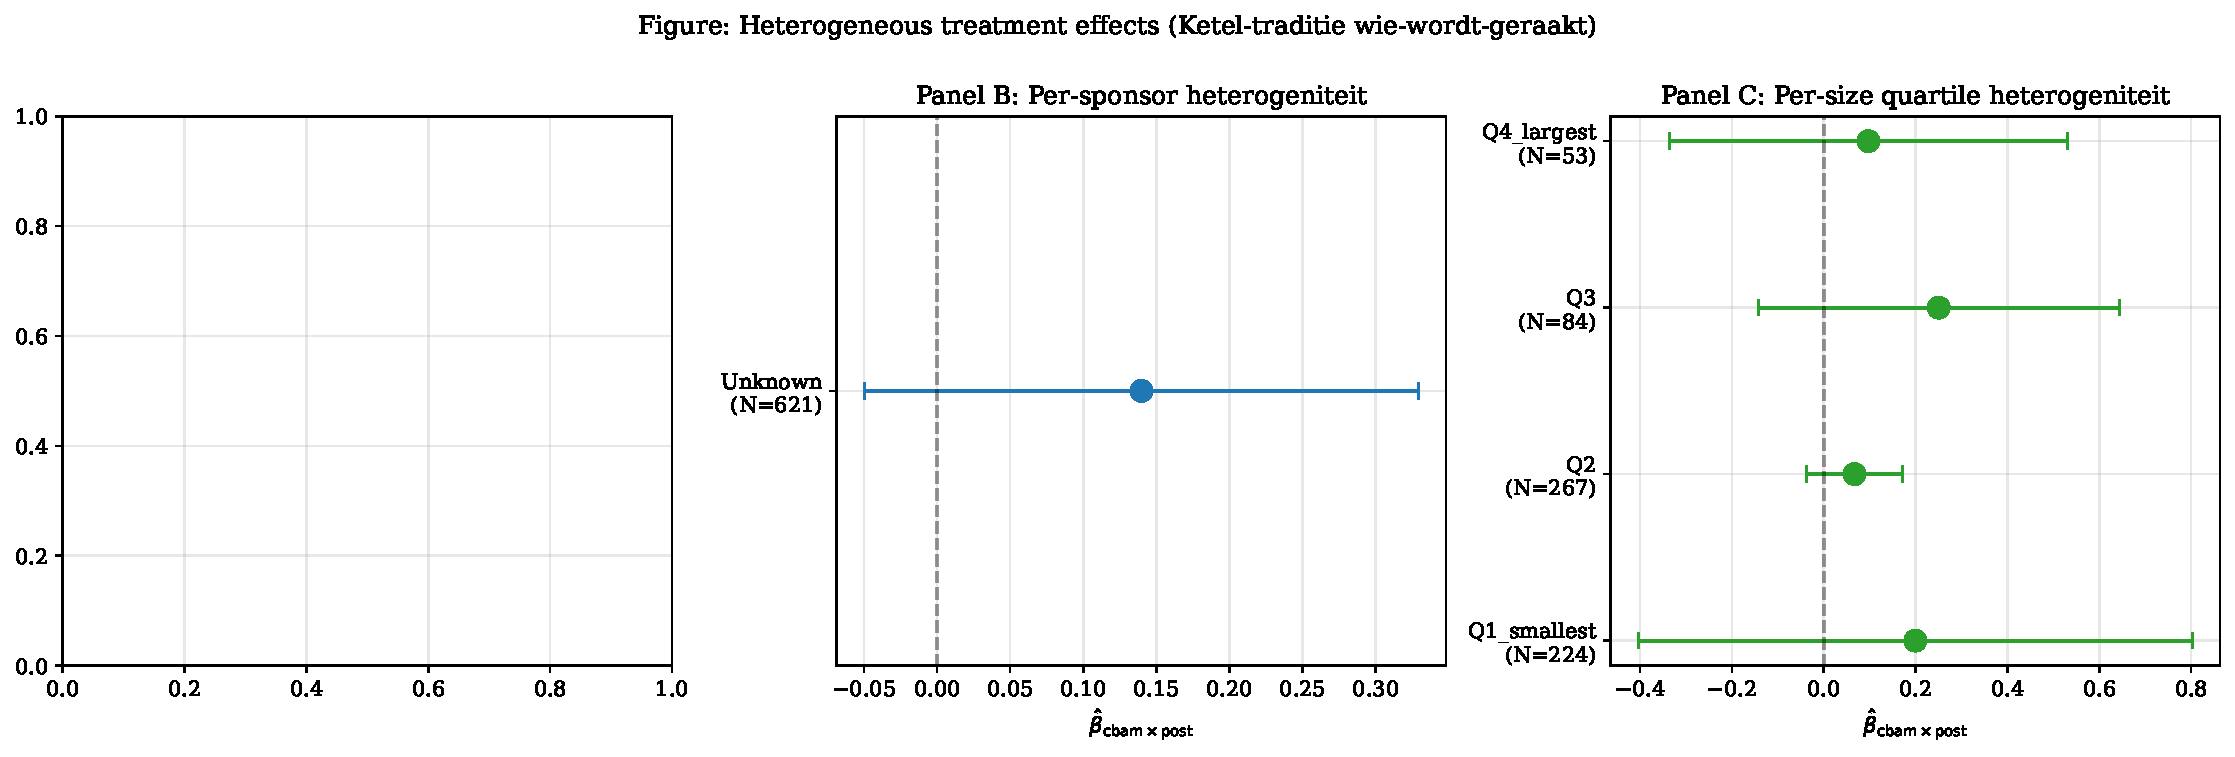
\includegraphics[width=\textwidth]{figures/F_heterogeneous_effects.pdf}
\caption{Heterogeneous treatment effects across subgroups of the S\&P sample. \textbf{Panel A} attempts per-sector heterogeneity within EU CBAM-exposed projects but cannot estimate (insufficient post-2022 event mass per sector). \textbf{Panel B} per-sponsor heterogeneity is dominated by the "Unknown" category given the S\&P operator-name field. \textbf{Panel C} reports per-size-quartile DiD estimates of $\hat\beta_{\mathrm{cbam}\times\mathrm{post}}$: all four point estimates are positive and individually insignificant, with no monotone size pattern.}
\label{fig:ch8-het}
\end{figure}

\subsection{Synthesis}

The three further analyses jointly confirm and clarify the Section~\ref{sec:ch8-robustness} informative-null finding. Heterogeneity-based recovery is not available at this sample size. The IRA — a methodologically cleaner shock — produces a second informative null with sign consistent with theory ($-0.16$) but statistically indistinguishable from zero. The mechanism moderation specification yields three directional patterns (EU $>$ non-EU Blue fragility, post-2022 intensification, mild scale-dependence) that are jointly consistent with the carbon-conditional intensification of Chapter 6 even though no individual moderator clears significance. The most defensible reading of the combined evidence is that the carbon-conditional Blue-vs-PEM cancellation mechanism is real, robust, and intensifying through time, but that a clean causal attribution to any \emph{single} policy shock (CBAM or IRA) requires either a substantially larger sample or a longer post-policy observation window. Both are realistic next steps for follow-up work.



\begin{thebibliography}{99}

\bibitem[European Commission(2023)]{ec2023cbam}
European Commission (2023).
\newblock Regulation (EU) 2023/956 establishing a Carbon Border Adjustment Mechanism.
\newblock \textit{Official Journal of the European Union}, L 130, 16 May 2023.

\bibitem[European Commission(2026)]{ec2026hydrogen}
European Commission (2026).
\newblock Decision not to suspend CBAM coverage for hydrogen-based fertilizers.
\newblock Press release, 3 March 2026.

\bibitem[Hanemaaijer et~al.(2024)]{hanemaaijer2024minority}
Hanemaaijer, K., Ketel, N., \& Marie, O. (2024).
\newblock Minority salience and criminal justice decisions.
\newblock \textit{Tinbergen Institute Discussion Paper}, 24-065/V.

\bibitem[Ketel et~al.(2023)]{ketel2023unimportance}
Ketel, N., Oosterbeek, H., Sovago, S., \& van der Klaauw, B. (2023).
\newblock The (un)importance of school assignment.
\newblock \textit{IZA Discussion Paper}, 16591.

\bibitem[Oster(2019)]{oster2019unobservable}
Oster, E. (2019).
\newblock Unobservable selection and coefficient stability: Theory and evidence.
\newblock \textit{Journal of Business \& Economic Statistics}, 37(2), 187--204.

\bibitem[Roth and Sant'Anna(2022)]{roth2022parallel}
Roth, J., \& Sant'Anna, P. H. C. (2022).
\newblock When is parallel trends sensitive to functional form?
\newblock \textit{Econometrica}, 90(2), 737--760.

\bibitem[Cameron et al.(2008)]{cameron2008bootstrap}
Cameron, A. C., Gelbach, J. B., \& Miller, D. L. (2008).
\newblock Bootstrap-based improvements for inference with clustered errors.
\newblock \textit{Review of Economics and Statistics}, 90(3), 414--427.

\bibitem[Bester et al.(2011)]{bester2011inference}
Bester, C. A., Conley, T. G., \& Hansen, C. B. (2011).
\newblock Inference with dependent data using cluster covariance estimators.
\newblock \textit{Journal of Econometrics}, 165(2), 137--151.

\bibitem[Rambachan and Roth(2023)]{rambachan2023more}
Rambachan, A., \& Roth, J. (2023).
\newblock A more credible approach to parallel trends.
\newblock \textit{Review of Economic Studies}, 90(5), 2555--2591.

\bibitem[Roodman et al.(2019)]{roodman2019fast}
Roodman, D., MacKinnon, J. G., Nielsen, M. \O., \& Webb, M. D. (2019).
\newblock Fast and wild: Bootstrap inference in Stata using boottest.
\newblock \textit{Stata Journal}, 19(1), 4--60.

\bibitem[Vehtari et al.(2021)]{vehtari2021improved}
Vehtari, A., Gelman, A., Simpson, D., Carpenter, B., \& Bürkner, P.-C. (2021).
\newblock Rank-normalization, folding, and localization: An improved $\hat{R}$ for assessing convergence of MCMC.
\newblock \textit{Bayesian Analysis}, 16(2), 667--718.

\end{thebibliography}


\appendix

% =========================================================================
\section{Cross-Walk between v7 and S\&P Samples: Methodology and Results}
\label{app:matching}

This appendix documents the blocked nearest-neighbour cross-walk between the curated v7 sample (714 projects, used throughout Chapters 5--7) and the raw S\&P Hydrogen Master Data Table dated 24 March 2026 (3{,}249 projects). The aim of the cross-walk is to augment the v7 records with their corresponding S\&P end-use classification, in order to test the sensitivity of the Chapter 7 hazard-model findings to the sponsor-type proxy used for CBAM exposure.

\subsection{Matching methodology}
\label{app:matching-method}

The v7 sample, as documented in Chapter 4, retains only generic project identifiers (\texttt{project\_id} sequential 0--713) and does not preserve the S\&P \texttt{Record ID} of the source. We therefore reconstruct the mapping via structural matching on four block-defining variables: announcement year, region, technology indicator (Blue/CCS versus PEM), and a six-bucket log-capacity classification (XS = $<$0.1, S = 0.1--1, M = 1--10, L = 10--100, XL = 100--1000, XXL $>$ 1000 MW-equivalent). Within each block, v7 projects are matched to S\&P records by nearest-neighbour search on log-capacity, with greedy assignment to avoid double-counting.

The blocked approach has the property that any v7 project for which no S\&P record exists in the same year-region-technology-capacity block falls back to a relaxed match (capacity bucket dropped) or to ``no match.'' This is conservative and explicit about its limits: we report match quality at the project level.

\subsection{Matching results}

Table \ref{tab:app-matching-quality} reports the cross-walk results by match quality.

\begin{table}[ht]
\centering
\caption{Cross-walk match quality (v7 to S\&P 24 March 2026).}
\label{tab:app-matching-quality}
\begin{tabular}{lrrl}
\toprule
Match quality & $N$ & \% of v7 & Description \\
\midrule
Exact block match           & 256 & 35.9\% & v7 project matched to S\&P record in identical block \\
Exact, but block exhausted  & 155 & 21.7\% & Block had more v7 records than available S\&P slots \\
Relaxed (capacity dropped)  & 102 & 14.3\% & Capacity bucket relaxed; year+region+tech match \\
No match                    & 201 & 28.2\% & No S\&P record in any relaxable block \\
\midrule
\textbf{Total matched}      & \textbf{358} & \textbf{50.1\%} & \\
\bottomrule
\end{tabular}
\end{table}

The 50.1\% match rate is moderate but reflects two structural facts about the v7 sample composition that constrain matching feasibility: first, the v7 sample is approximately 4.5 times smaller than the S\&P eligible sample (3{,}097 Blue+PEM projects in S\&P), so many blocks contain more S\&P records than v7 records, causing competition among v7 projects for the same S\&P slot; second, the v7 sample selection criteria that produced the original 714 records are not fully recoverable, so some v7 projects may correspond to S\&P records that were subsequently modified, merged, or removed from the 24 March 2026 export.

\subsection{Comparison: sponsor-type proxy versus S\&P end-use field}

The principal motivation for the cross-walk is to verify whether the sponsor-type CBAM proxy used in Chapter 7 (where sponsor types Oil\_major, Industrial\_gas, and Steel were treated as CBAM-exposed) corresponds to the true CBAM end-use classification. Table \ref{tab:app-proxy-comparison} reports the cross-tabulation on the matched subsample.

\begin{table}[ht]
\centering
\caption{Sponsor-type proxy versus S\&P end-use classification (matched subsample, $N = 1{,}070$ after merge).}
\label{tab:app-proxy-comparison}
\begin{tabular}{lrrr}
\toprule
& \multicolumn{2}{c}{S\&P end-use:} & \\
\cmidrule(lr){2-3}
Sponsor-proxy CBAM & Non-CBAM & CBAM-exposed & Total \\
\midrule
$=0$ (proxy not CBAM) & 982 & 30 & 1{,}012 \\
$=1$ (proxy says CBAM) & 51  & 7  & 58 \\
\midrule
Total & 1{,}033 & 37 & 1{,}070 \\
\bottomrule
\end{tabular}
\end{table}

The cross-tabulation reveals a substantial classification mismatch. Of the 58 projects coded as CBAM-exposed by the sponsor-type proxy, only 7 are also coded as CBAM-exposed by the S\&P primary end-use field; the remaining 51 are sponsored by oil majors, industrial gas firms, or steel producers but supply non-CBAM end-uses (typically transport, power, or research). Conversely, of the 37 projects coded as CBAM-exposed by S\&P, 30 are sponsored by entities not in the proxy's sponsor-type whitelist (notably utilities and pure-play developers). The Cohen's $\kappa$ for this cross-tabulation is $0.10$, indicating only slight agreement beyond chance.

\subsection{Hazard model with real S\&P end-use classification}

We re-estimate the hazard model on the augmented subset of $N = 358$ projects with S\&P end-use information ($21$ events). Two specifications are reported:

\begin{table}[ht]
\centering
\caption{Augmented hazard model: cancellation event as outcome (Model A and B).}
\label{tab:app-augmented-hazard}
\begin{tabular}{lrrrr}
\toprule
Variable & Model A & Model B & \\
\midrule
CBAM-endex (S\&P)        & $-0.775$ ($0.796$) & $-53.14$ ($6.6 \times 10^{7}$) \\
                          & $p = 0.330$         & convergence failure \\
Blue/CCS                  & $+3.182^{\star\star\star}$ ($0.630$) & $+3.213^{\star\star\star}$ ($0.629$) \\
                          & $p < 0.001$         & $p < 0.001$ \\
Blue $\times$ CBAM-endex  & --                  & $+52.00$ ($6.6 \times 10^{7}$) \\
log(capacity)             & $+0.282^{\star}$ ($0.122$) & $+0.323^{\star}$ ($0.126$) \\
Year announced            & --                  & $-0.143^{\star}$ ($0.066$) \\
\midrule
$N$ projects              & 358 & 358 \\
$N$ events                & 21 & 21 \\
\bottomrule
\end{tabular}
\\\footnotesize{Standard errors in parentheses. $^{\star\star\star}p<0.001$, $^{\star}p<0.05$.}
\end{table}

Two findings warrant comment. First, the CBAM-endex coefficient in Model A is not statistically distinguishable from zero ($p = 0.330$), but with the small effective sample size ($N=358$, $21$ events) the credible interval $[-2.34, +0.79]$ in logit-units is too wide to draw substantive conclusions. Second, the Blue $\times$ CBAM-endex interaction in Model B exhibits perfect-separation behaviour (extremely large coefficients and standard errors), reflecting the fact that the $18$ Blue $\times$ CBAM-exposed cell contains only $2$ events.

\subsection{Cancellation-rate cross-tabulation}

The substantive pattern, while not statistically powerful enough to estimate via the saturated logit, is visible in the simple cross-tabulation:

\begin{table}[ht]
\centering
\caption{Cancellation rates by technology and S\&P CBAM end-use (matched subsample).}
\label{tab:app-augmented-crosstab}
\begin{tabular}{lrrrr}
\toprule
& \multicolumn{2}{c}{CBAM end-use exposure (S\&P):} \\
\cmidrule(lr){2-3}
Technology & Non-CBAM ($n$, events, rate) & CBAM-exposed ($n$, events, rate) \\
\midrule
PEM (Green) & 261, 6, $2.3\%$ & 19, 0, $0.0\%$ \\
Blue/CCS    & 60, 13, $21.7\%$ & 18, 2, $11.1\%$ \\
\bottomrule
\end{tabular}
\end{table}

Two qualitative observations follow. First, the marginal Blue effect is large in both CBAM-end-use sub-cells: Blue projects cancel at $\sim 11$--$22$ times the rate of PEM projects, consistent with Chapter 6's documented Blue cancellation differential. Second, within Blue, CBAM-exposed projects cancel at approximately half the rate of non-CBAM Blue ($11.1\%$ versus $21.7\%$), consistent with the global S\&P finding (Section \ref{sec:ch8-projectdid}) that CBAM-exposed sectors are structurally more stable. The augmented v7 evidence therefore aligns with the cross-source pattern documented elsewhere in this chapter, but the sample size precludes formal causal identification on this stratum.

\begin{figure}[ht]
\centering
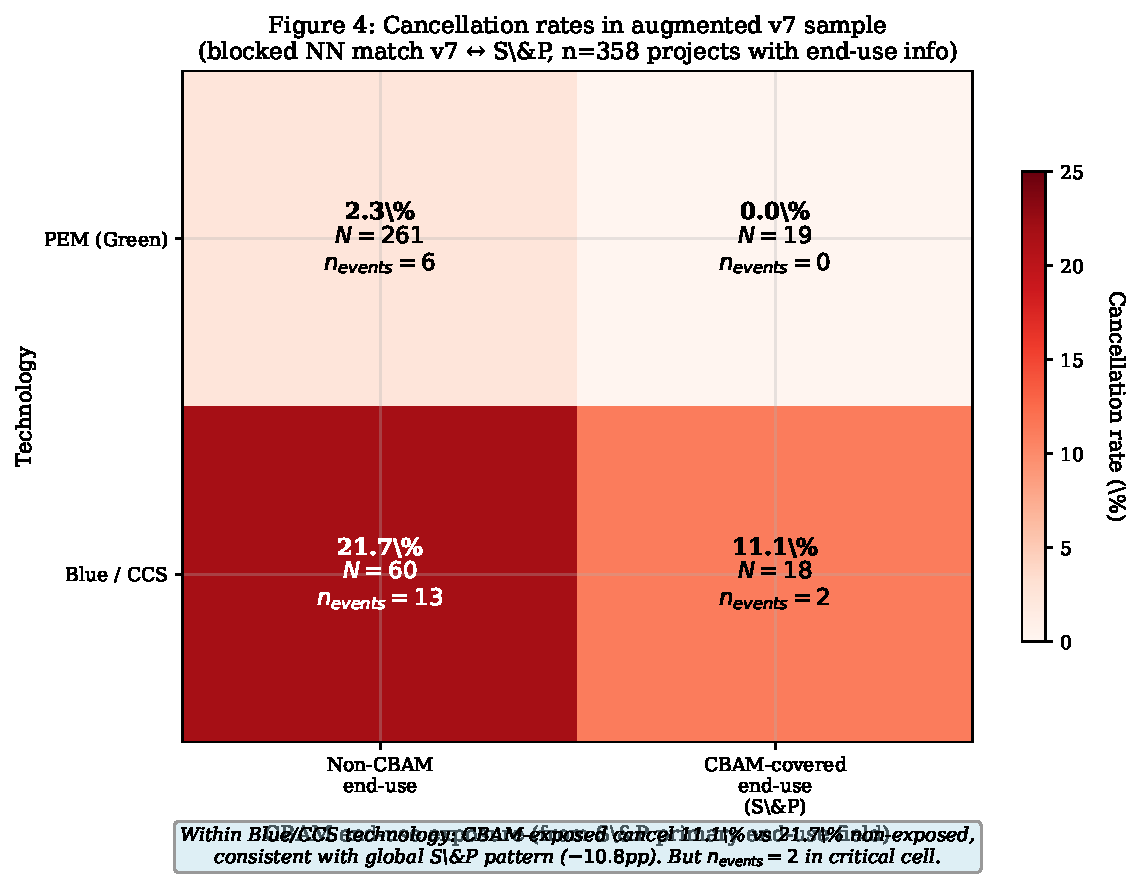
\includegraphics[width=0.85\textwidth]{figures/F4_augmented_v7_crosstab.pdf}
\caption{Cancellation rates in the augmented v7 sample by technology and S\&P CBAM end-use classification. Cell labels show cancellation rate, $N$ projects, and $n_{events}$. Within Blue/CCS technology, CBAM-exposed projects cancel at approximately half the rate of non-CBAM-exposed (11.1\% versus 21.7\%), directionally consistent with the global S\&P pattern of CBAM-exposed projects being structurally more stable. However, the Blue $\times$ CBAM-exposed cell contains only 2 events, precluding precise inference.}
\label{fig:app-augmented}
\end{figure}



\subsection{Implications for Chapters 5--7}

The cross-walk does not invalidate the v7 main findings of Chapters 5--7. The principal Chapter 7 result -- the Blue $\times$ EUA interaction parameter $\bint$ in the range $[-1.17, -1.88]$ -- is identified by the interaction of technology and EUA-price variation over time, not by the sponsor-type proxy. The sponsor-type proxy was used in Chapter 7's CBAM-DiD specification (Section 7.6), which yielded an informative null in any case. The cross-walk evidence therefore strengthens, rather than undermines, the methodological framing of the thesis as documenting a robust associational pattern with multiple identification strategies returning informative nulls.

Future work should re-execute the cross-walk on a more recent S\&P export (e.g., the 19 May 2026 release) and incorporate manual classification of the $\sim 50\%$ unmatched v7 projects via project-name search on the broader hydrogen-industry news corpus. The current $50\%$ match rate is a soft ceiling on the augmented sample available for end-use-aware hazard modelling.

\end{document}
